\documentclass[11pt]{article}
\usepackage[T1]{fontenc}
\usepackage{lmodern}
\usepackage[margin=1in]{geometry}
\usepackage{amsmath,amssymb,amsthm,mathtools,microtype}
\usepackage{tikz}
\usetikzlibrary{arrows.meta}
\usepackage{xurl}
\usepackage[hidelinks,pdfusetitle]{hyperref}
\newcommand{\R}{\mathbb R}
\newcommand{\eps}{\varepsilon}
\newcommand{\area}{\operatorname{area}}
\newcommand{\norm}[1]{\lVert#1\rVert}
\newtheorem{theorem}{Theorem}[section]
\newtheorem{lemma}[theorem]{Lemma}
\newtheorem{proposition}[theorem]{Proposition}
\newtheorem{corollary}[theorem]{Corollary}
\theoremstyle{remark}
\newtheorem{remark}[theorem]{Remark}
\numberwithin{equation}{section}
\setlength{\emergencystretch}{2em}
\title{Finite triangular approximation of radial sweeps}
\author{OpenAI}
\date{September 27, 2026}
\begin{document}
\maketitle
\begin{abstract}
We prove that radially aligned segment sweeps admit finite cylinder
covers with one triangular base for each interval of any tagged
partition. As the mesh tends to zero, the total perpendicular base area
converges to a weighted parameter area. An explicit application covers every
regular
tetrahedron with total base area below half its minimum projection area,
giving negative answers to the half-area question and the directionwise
normalized 1-Codimensional Cylinder Covering Conjecture.
\end{abstract}
\section{Radial sweeps and finite cylinders}
\label{sec:introduction}

A cylinder in $\R^3$ is a set $B+\R u$, where $u$ is a unit vector
and $B\subset u^\perp$ is a measurable planar set of finite area.
Its cost is $\area(B)$. In a finite cover, the costs are added with
multiplicity. For a convex body $K$, write
\[
 A_{\min}(K)=\min_{\norm{u}=1}\area(\pi_{u^\perp}K).
\]
The half-area question asks whether every finite cylinder cover of $K$
has cost at least $A_{\min}(K)/2$. A regular tetrahedron has a simple
cover by two opposite-edge cylinders attaining this value.
A second covering quantity is the directionwise normalized cost
\[
 \sum_i\frac{\area(B_i)}{\area(\pi_{u_i^\perp}K)},
\]
which divides each base area by the shadow in its own axis direction.

These questions extend plank covering, where the cost of a covering
slab is its width rather than the area of a planar base. Bezdek's
Problem~3.1 attributes the half-area question and the tetrahedral
equality example to Bang~\cite{Bezdek2009}.
Bezdek and Litvak prove that the directionwise normalized cost is at
least \(1/3\) for every three-dimensional convex body and at least \(1\)
for ellipsoids~\cite[Theorem~3.1]{BL2009}. In dimension three, Bezdek
and Khan's \emph{1-Codimensional Cylinder Covering Conjecture} proposes
the lower bound \(1/2\) for all convex bodies
\cite[Definition~3 and Conjecture~4.13]{BK2016}.
Such a normalized bound would imply the half-minimum bound, since
each directional projection area is at least \(A_{\min}(K)\).
The half-area question also appears in Verreault's survey
\cite[Question~4.14]{Verreault2026}. Our construction lowers the
tetrahedron's two-cylinder cost strictly by varying the directions,
while keeping coverage after finite approximation.

Our approximation problem begins before the cylinders are selected.
Let $P$ be a two-dimensional Euclidean plane through the origin, and
let $e$ be a unit normal to $P$. Choose linearly independent
$a,b\in P$, an interval $J=[\alpha,\beta]$ with $\alpha<\beta$,
a continuous function $R:J\to[0,\infty)$, and a continuously
differentiable function $w:J\to P$. With $p_0\in P$ and $L>0$,
consider the compact set
\begin{equation}\label{eq:radial-sweep}
 \mathcal S=\{p_0+\rho(a+tb)+s(e+w(t)):
          t\in J,\ 0\le\rho\le R(t),\ |s|\le L\}.
\end{equation}
At each $t$, the intercepts form one radial segment in $P$ and the
parallel swept segments have direction $e+w(t)$. The direction varies
with $t$, so this description is not yet a finite cylinder cover.

Put $\kappa=|\det_P(a,b)|$, the area of their parallelogram.
The radial parameterization has area element $\kappa\rho\,d\rho\,dt$.
Projection onto the plane perpendicular to $e+w(t)$ contributes
the factor $(1+\norm{w(t)}^2)^{-1/2}$. These two factors suggest the
weighted area
\begin{equation}\label{eq:weighted-area}
 \mathcal A=\kappa\int_\alpha^\beta
       \frac{R(t)^2}{2\sqrt{1+\norm{w(t)}^2}}\,dt.
\end{equation}
Freezing arbitrary segment directions need not preserve this cost.
The following alignment condition makes the loss vanish.

\begin{theorem}\label{thm:radial}
For the data in \eqref{eq:radial-sweep}, suppose that
\[
 w'(t)=\lambda(t)(a+tb)\qquad(t\in J)
\]
for a continuous real function $\lambda$.
For any finite partition
\(\alpha=t_0<t_1<\cdots<t_N=\beta\), put \(I_i=[t_{i-1},t_i]\)
and choose arbitrary tags \(c_i\in I_i\). There are \(N\) cylinders
covering \(\mathcal S\), with axes parallel to \(e+w(c_i)\) and
nondegenerate compact triangular perpendicular bases. These covers
can be chosen so that their total base area tends to \(\mathcal A\)
as the mesh \(\delta=\max_i|I_i|\) tends to zero, uniformly over the
partitions and tags.

Alternatively, take each base to be the perpendicular projection of
the actual compact sweep with \(t\in I_i\), in the same frozen
direction \(e+w(c_i)\). These \(N\) cylinders cover \(\mathcal S\),
and their total base area also tends to \(\mathcal A\), uniformly
over the partitions and tags.
\end{theorem}

The hypothesis has a direct geometric meaning. To first order, a
change in direction moves the intercept along its existing ray.
After that displacement is absorbed into the radial coordinate, the
remaining transverse displacement is quadratic in the interval length.
A slightly extended triangle contains all these intercepts and adds
only a vanishing total area. The radial cap $R$ may vanish, and
$\lambda$ may change sign or vanish.

The tetrahedral application gives the following concrete consequence.
\begin{corollary}\label{cor:tetrahedron}
Every regular tetrahedron $K\subset\R^3$ of positive edge length has
a finite cylinder cover $B_i+\R u_i$, with unit axes $u_i$ and
nondegenerate compact triangular bases $B_i\subset u_i^\perp$, such that
\[
 \sum_i\area(B_i)<\frac{A_{\min}(K)}2,
 \qquad
 \sum_i\frac{\area(B_i)}{\area(\pi_{u_i^\perp}K)}<\frac12.
\]
\end{corollary}

There is a useful connection with finite approximation for velocity
fields having square-zero derivative. Away from the apex, write
$z=\rho(a+tb)$ with $\rho>0$ and $t\in(\alpha,\beta)$, and define
$W(z)=w(t)$. This is a $C^1$ field in the open angular sector.
The angular differential $Dt$ annihilates $a+tb$, whereas
$DW=w'(t)\otimes Dt$. The alignment hypothesis therefore gives
$(DW)^2=0$. General finite approximation for such fields concerns a
larger class of ruled sets; see the companion article
\cite[Theorem~1.2 and Section~3]{RuledApproximation2026}. Theorem~\ref{thm:radial} proves the
simultaneous prescribed-tag, one-cylinder-per-interval and triangular-base
guarantee directly, including the apex. Merely splitting parallelogram
bases into triangles would not preserve that prescribed count and choice
of axes. No approximation theorem for general velocity fields is used here.

The proof of Theorem~\ref{thm:radial} in
Section~\ref{sec:freezing} constructs the enclosing triangles and
bounds their total excess area. The actual projected sweep contains
the projection of the unperturbed radial sector, which supplies the matching lower
bound. Thus different finite bases have the same limiting cost.

Section~\ref{sec:tetrahedron} proves Corollary~\ref{cor:tetrahedron}
with two overlapping sweeps. A cubic enlargement of their radial caps
exceeds the uniform error in selecting a segment through each point,
while a negative quadratic projection cost survives finite
approximation. Section~\ref{beam:section} develops the alternative
shortened-beam construction: the beam saving and the residual-strip
cost cancel to first order, leaving a strict quadratic improvement.
Its quantitative cost statement separates this construction from the
all-triangular cover already obtained.

The appendices collect supplementary calculations and alternative
finite bases. Appendix~\ref{sec:projections} gives simplex projection
normalizations. Appendix~\ref{sec:cap-choices} compares overlap
margins, Appendix~\ref{sec:finite-footprints} computes explicit finite
enclosures, and Appendix~\ref{sec:coordinate-realizations} transports
the construction between physical and barycentric coordinates.
These calculations retain their own formulas and geometric
realizations; neither main construction requires them.

\section{A triangle around each frozen intercept}
\label{sec:freezing}

We prove Theorem~\ref{thm:radial}. The required estimate is local to
one interval, but its error must be uniform over the whole partition.
Set
\[
 M=\max_J|\lambda|,\qquad A=LM,\qquad B=LM/2.
\]
Take any finite partition $\alpha=t_0<t_1<\cdots<t_N=\beta$.
For each interval $I=[t_{j-1},t_j]$, put $d_I=|I|$, let $m_I$ be
its midpoint, and set $R_I=\max_I R$. Write
$\delta=\max_I d_I$ for the mesh. The freezing tag $c_I\in I$
need not be the midpoint.

Move a point of \eqref{eq:radial-sweep} with $t\in I$ parallel to
$e+w(c_I)$ until it reaches $P$. Its intercept is
\[
 p_0+\rho(a+tb)+s(w(t)-w(c_I))=p_0+u a+v b,
\]
where, using the derivative hypothesis,
\begin{align}
 u&=\rho+s\int_{c_I}^t\lambda(\xi)\,d\xi,
 \label{eq:radial-coordinate}\\
 v-tu&=s\int_{c_I}^t\lambda(\xi)(\xi-t)\,d\xi.
 \label{eq:transverse-error}
\end{align}
Consequently
\begin{equation}\label{eq:old-footprint}
 -Ad_I\le u\le R_I+Ad_I,\qquad
 |v-m_Iu|\le\frac{d_I}{2}|u|+Bd_I^2.
\end{equation}
The first inequality uses $|t-c_I|\le d_I$; the second also uses
$|t-m_I|\le d_I/2$. In particular, the error transverse to a ray
is of order $d_I^2$, even though $u$ can move by order $d_I$ and can
become negative.

To enclose both the transverse error and the negative radial collar,
choose $C=2(A+B)+1$. Define the triangle in $P$
\begin{equation}\label{eq:triangle}
 T_I=\left\{p_0+u a+v b:
 -Cd_I\le u\le R_I+Ad_I,\quad
 |v-m_Iu|\le\frac{d_I}{2}(u+Cd_I)\right\}.
\end{equation}
Its width is zero at $u=-Cd_I$ and is positive at $u=R_I+Ad_I$.
Since $R_I+(A+C)d_I>0$, it is nondegenerate, including when $R_I=0$.

The triangle contains every intercept in
\eqref{eq:old-footprint}. The radial ranges are nested because
$C>A$. For $u\ge0$ the difference between the new half-width and
$d_I|u|/2$ is $Cd_I^2/2\ge Bd_I^2$. For $-Ad_I\le u<0$, that
difference is
\[
 d_Iu+\frac C2d_I^2\ge\left(\frac C2-A\right)d_I^2\ge Bd_I^2.
\]
This proves containment on both sides of the original radial tip;
Figure~\ref{fig:triangle} illustrates that extension.

\begin{figure}[htbp]
\centering
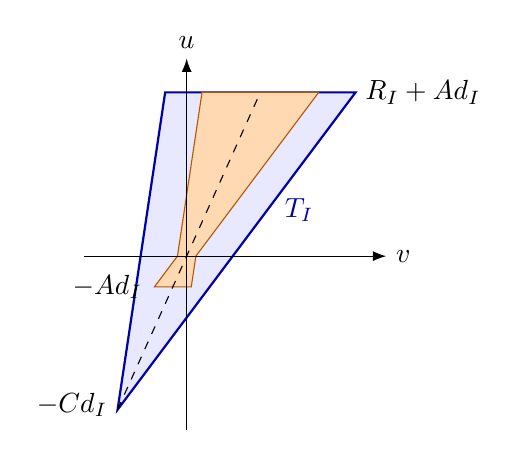
\begin{tikzpicture}[scale=1.3]
 \fill[blue!9] (-.675,-1.5)--(-.21,1.6)--(1.65,1.6)--cycle;
 \draw[blue!65!black,thick] (-.675,-1.5)--(-.21,1.6)--(1.65,1.6)--cycle;
 \fill[orange!30] (-.315,-.3)--(-.09,0)--(.15,1.6)--(1.29,1.6)--(.09,0)--(.045,-.3)--cycle;
 \draw[orange!70!black] (-.315,-.3)--(-.09,0)--(.15,1.6)--(1.29,1.6)--(.09,0)--(.045,-.3)--cycle;
 \draw[dashed] (-.675,-1.5)--(.72,1.6);
 \draw[-{Latex}] (-1,0)--(1.95,0) node[right] {$v$};
 \draw[-{Latex}] (0,-1.7)--(0,1.93) node[above] {$u$};
 \node[left] at (-.68,-1.45) {$-Cd_I$};
 \node[left] at (-.34,-.3) {$-Ad_I$};
 \node[right] at (1.65,1.6) {$R_I+Ad_I$};
 \node[blue!65!black] at (1.1,.45) {$T_I$};
\end{tikzpicture}
\caption{In intercept coordinates, the orange polygon bounds the
frozen sweep, including the small region below $u=0$. The enclosing
blue triangle extends its tip to $u=-Cd_I$; the dashed line is
$v=m_Iu$. The drawing is schematic; the triangle and footprint are
defined by \eqref{eq:triangle} and \eqref{eq:old-footprint}.}
\label{fig:triangle}
\end{figure}


Let $v_I=e+w(c_I)$ and take the base
$B_I=\pi_{v_I^\perp}T_I$. The restriction of this projection to
$P$ is nonsingular: its unit normal component is
$|e\cdot v_I|/\norm{v_I}=1/\norm{v_I}>0$.
Thus $B_I$ is again a nondegenerate compact triangle.
Moreover, $T_I+\R v_I=B_I+\R v_I$, since a point and its
orthogonal projection differ by a multiple of $v_I$.
The containment already proved shows that these cylinders cover
$\mathcal S$.

The area factor of projection from $P$ is $1/\norm{v_I}$.
Indeed, an orthonormal basis of $P$ projects to a parallelogram
whose area is the absolute scalar product of $e$ and
$v_I/\norm{v_I}$. The coordinate change $(u,v)\mapsto u a+v b$
has area factor $\kappa$. Integrating the width of
\eqref{eq:triangle} therefore gives the exact formula
\begin{equation}\label{eq:triangle-area}
 \area(B_I)=
 \frac{\kappa d_I\,[R_I+(A+C)d_I]^2}
      {2\sqrt{1+\norm{w(c_I)}^2}}.
\end{equation}
The collar changes $d_IR_I^2/2$ by $O(d_I^2)$, uniformly over $I$,
because $R$ is bounded. Since
$\sum_I d_I^2\le\delta(\beta-\alpha)$, its total contribution tends
to zero with the mesh. Put
$g(t)=(1+\norm{w(t)}^2)^{-1/2}$. Uniform continuity of $R$ and $g$
then gives
\[
 \sum_I\frac{\kappa d_I R_I^2g(c_I)}2
 \longrightarrow\frac\kappa2\int_J R(t)^2g(t)\,dt=\mathcal A.
\]
Thus the triangular covers have the asserted limit for arbitrary
partitions and tags. No convergence rate for the entire sum is needed
or asserted for an arbitrary continuous $R$.

For the actual projected bases, let $\mathcal S_I$ be the compact
sweep with $t\in I$, and put $B_I^{\mathrm{act}}=\pi_{v_I^\perp}\mathcal S_I$.
Moving parallel to $v_I$ does not change this projection, so the
intercept containment already proved gives $B_I^{\mathrm{act}}\subseteq B_I$.
The set $B_I^{\mathrm{act}}$ is compact and its cylinder contains
$\mathcal S_I$.

A matching lower bound comes from the sector at $s=0$:
\[
 E_I=\{p_0+\rho(a+tb):t\in I,\ 0\le\rho\le R(t)\}
 \subseteq\mathcal S_I.
\]
In the $(a,b)$ coordinates this map is $(\rho,t)\mapsto(\rho,\rho t)$,
which is one-to-one for $\rho>0$ and has absolute Jacobian $\rho$.
The edge $\rho=0$ maps to a single point. Consequently
$\area(E_I)=\frac\kappa2\int_I R(t)^2\,dt$, and projection from $P$
scales this area by $g(c_I)$. We obtain the two-sided estimate
\begin{equation}\label{eq:actual-sweep-squeeze}
 \frac{\kappa g(c_I)}2\int_I R(t)^2\,dt
 \le\area(B_I^{\mathrm{act}})\le\area(B_I).
\end{equation}
The sum of the lower bounds tends to $\mathcal A$: its difference
from the integral is at most
\[
 \frac\kappa2\sup_{\substack{r,t\in J\\|r-t|\le\delta}}
 |g(r)-g(t)|\int_J R(t)^2\,dt,
\]
which tends to zero by uniform continuity. The upper sums have the
same limit, proving the actual-base assertion, including when $R$
vanishes. This shared limit does not identify the individual actual
bases with their containing triangles or make their finite areas equal.
The proof of Theorem~\ref{thm:radial} is complete.

\section{Two overlapping sweeps in a tetrahedron}
\label{sec:tetrahedron}

We now choose two sweeps for which the weighted cost is strictly
smaller than the half-area bound. Write physical points as
$(x,y,ht)$, where $h=\sqrt2$, and let
\begin{equation}\label{eq:tetrahedron}
 K=\{(x,y,ht):|x|\le1+t,\ |y|\le1-t\}.
\end{equation}
The inequalities imply $-1\le t\le1$. The four vertices are
$(\pm2,0,h)$ and $(0,\pm2,-h)$, and their pairwise distances
are four. This is a regular tetrahedron.

\subsection{The reference area}

For a polytope with face areas $S_j$, outward unit normals $n_j$,
and a unit vector $u$, Cauchy's projection formula takes the form
\begin{equation}\label{eq:cauchy}
 \area(\pi_{u^\perp}K)=\frac12\sum_j S_j|n_j\cdot u|.
\end{equation}
See Martini \cite[p.~83, equation~(1)]{Martini1991} for the
projection-body formulation. The elementary polytope proof is to
count the two endpoints of almost every line parallel to $u$:
projecting all faces counts its shadow twice, whereas edges and
faces parallel to $u$ contribute zero area.

Each face of \eqref{eq:tetrahedron} has area $4\sqrt3$, and its
normal is one of the normalizations of
$(\pm1,0,-1/h)$ and $(0,\pm1,1/h)$.
For a unit vector $u=(u_1,u_2,u_3)$, formula~\eqref{eq:cauchy}
and $|a+b|+|a-b|=2\max(|a|,|b|)$ give
\[
 \area(\pi_{u^\perp}K)
 =4h\left(\max\{|u_1|,|u_3|/h\}
          +\max\{|u_2|,|u_3|/h\}\right).
\]
If the two maxima are $X,Y$, then
$X^2+Y^2\ge u_1^2+u_2^2$ and $XY\ge u_3^2/h^2$.
Since $h^2=2$, it follows that $(X+Y)^2\ge1$.
Equality is attained at $u=(1,0,0)$, so
\begin{equation}\label{eq:min-area}
 A_{\min}(K)=4h.
\end{equation}
The upper half of $K$ is covered by an $x$-parallel cylinder of
base area $h$, and the lower half by a $y$-parallel cylinder of
the same area. Their total cost is $2h=A_{\min}(K)/2$.

\subsection{The perturbed segments cover the whole tetrahedron}

For $q\in[-1,1]$, define
\[
 G(q)=\frac{1+q^2}{2},\qquad H(q)=\frac{q^2+q^4}{2},\qquad
 R_\eps(q)=1+\eps^2\bigl(H(q)+5\eps\bigr),\quad \eps>0.
\]
The upper sweep is
\begin{equation}\label{eq:upper-sweep}
 U_\eps=\{(x,\rho q-\eps xG(q),
                     h(1-\rho+\eps xq)):
       |x|\le2,\ |q|\le1,\ 0\le\rho\le R_\eps(q)\}.
\end{equation}
Its intercept ray starts at $(0,0,h)$ in direction $(0,q,-h)$.
The identity $G'(q)=q$ makes the derivative of its segment direction
$(1,-\eps G(q),h\eps q)$ equal to $-\eps(0,q,-h)$, exactly
the radial alignment required by Theorem~\ref{thm:radial}.
The constant term in $G$ gives
$G(q)-q^2=(1-q^2)/2$, which vanishes at both angular endpoints.
This will keep the endpoint levels unchanged when we select a line
through a point of $K$.

The sweep is compact. Let $\mathcal R(x,y,z)=(y,-x,-z)$, an orthogonal
map preserving $K$. Its image $\mathcal R U_\eps$ is the lower
sweep, which can equivalently be written as
\begin{equation}\label{eq:lower-sweep}
 \{(\sigma p+\eps yG(p),y,h(-1+\sigma+\eps yp)):
       |y|\le2,\ |p|\le1,\ 0\le\sigma\le R_\eps(p)\}.
\end{equation}
Indeed, apply $\mathcal R$ in \eqref{eq:upper-sweep} and replace
its free coordinate $x$ by $-y$. We will show that the two sweeps
overlap enough to cover $K$.

\begin{lemma}\label{lem:crossing}
If $F\in C^1([a,b])$, $a<b$, and $F(a)\le z\le F(b)$,
there is $r\in[a,b]$ with $F(r)=z$ and $F'(r)\ge0$,
using one-sided derivatives at the endpoints.
\end{lemma}
\begin{proof}
If $F(a)=z$ and $F'(a)\ge0$, use $r=a$.
Otherwise $F$ is below $z$ either at $a$ or immediately to its
right. Starting at such a point, take the first subsequent point
where $F=z$; it exists because $F(b)\ge z$. Its left difference
quotients are nonnegative, so its derivative is nonnegative.
\end{proof}

\begin{proposition}\label{prop:coverage}
For every $\eps>0$, the compact sets $U_\eps$ and
$\mathcal R U_\eps$ cover $K$.
\end{proposition}
\begin{proof}
Fix $(x,y,ht)\in K$. Applying Lemma~\ref{lem:crossing} twice
gives $q,p\in[-1,1]$ satisfying
\begin{align}
 y&=(1-t)q-\eps x(1-q^2)/2,
 &\rho&=1-t+\eps xq\ge0,\label{eq:root-one}\\
 x&=(1+t)p+\eps y(1-p^2)/2,
 &\sigma&=1+t-\eps yp\ge0.\label{eq:root-two}
\end{align}
In each equation the endpoint values bracket the coordinate on
the left, and the derivative is precisely the indicated radial
parameter. This includes zero-height slices and boundary points.
Rearranging gives the segment representations
\eqref{eq:upper-sweep} and \eqref{eq:lower-sweep}; only their
upper radial bounds remain to be checked.

If both bounds failed, then
\begin{equation}\label{eq:joint-failure}
 \eps yp+\eps^2(H(p)+5\eps)<t
       <\eps xq-\eps^2(H(q)+5\eps).
\end{equation}
As $|x|,|y|\le2$ and both cap corrections are nonnegative,
$|t|\le2\eps$. Equations~\eqref{eq:root-one}--\eqref{eq:root-two}
then imply
\[
 |x-p|\le3\eps,\qquad |y-q|\le3\eps.
\]
Moreover, \eqref{eq:joint-failure} puts $t/\eps$ between
$yp$ and $xq$. Both differ from $pq$ by at most $3\eps$, so
\begin{equation}\label{eq:interface-error}
 |t/\eps-pq|\le3\eps.
\end{equation}

Put $D(r)=(1-r^2)/2$, so $0\le D(r)\le1/2$ on $[-1,1]$.
The root equations give the exact identity
\[
 \frac{xq-yp}{\eps}
   =2pq\frac t\eps+yqD(p)+xpD(q).
\]
Replacing $t/\eps$ by $pq$ costs at most $6\eps$, by
\eqref{eq:interface-error}. Replacing $y$ by $q$ and $x$ by
$p$ costs at most $3\eps$ in total. Hence
\begin{align*}
 \frac{xq-yp}{\eps}
 &\le2p^2q^2+q^2D(p)+p^2D(q)+9\eps\\
 &=\frac{p^2+q^2}{2}+p^2q^2+9\eps.
\end{align*}
This is why the cap contains $H(q)=q^2G(q)$: the inequality
$2p^2q^2\le p^4+q^4$ gives
\[
 \frac{p^2+q^2}{2}+p^2q^2\le H(p)+H(q).
\]
The two cubic cap corrections contribute $10\eps$ after division
by $\eps^2$, exceeding the error $9\eps$.
Indeed, \eqref{eq:joint-failure} requires $(xq-yp)/\eps$ to be
strictly greater than $H(p)+H(q)+10\eps$. This contradiction
proves the proposition. All estimates were uniform over the closed
tetrahedron.
\end{proof}

\subsection{Finite bases and the weighted cost}

We now hold $\eps$ fixed. In the intercept plane $P=\{x=0\}$,
the upper sweep has the data
\[
 p_0=(0,0,h),\quad e=(1,0,0),\quad
 a=(0,0,-h),\quad b=(0,1,0),\quad L=2,
\]
and
\[
 w(q)=(0,-\eps G(q),h\eps q),\qquad
 w'(q)=-\eps(a+qb).
\]
Thus the hypothesis of Theorem~\ref{thm:radial} holds with
$\lambda=-\eps$, $\kappa=h$, and radial cap $R_\eps$.
Also
\[
 \norm{e+w(q)}^2=1+\eps^2D_0(q),\qquad
 D_0(q)=G(q)^2+2q^2.
\]
For every partition into $N$ intervals, the theorem and the orthogonal
map $\mathcal R$ cover $K$ by $2N$ cylinders with nondegenerate compact
triangular bases. As the mesh tends to zero, their total areas converge to
\begin{equation}\label{eq:cost-integral}
 2hI(\eps),\qquad
 I(\eps)=\int_{-1}^1
       \frac{R_\eps(q)^2}{2\sqrt{1+\eps^2D_0(q)}}\,dq.
\end{equation}
Taking actual swept projections instead gives compact bases with
the same limiting total area, for any choice of freezing tags.
Their finite areas may differ from those of the triangles.

\subsection{The saving and the final finite choice}

It remains to put the limiting cost strictly below $2h$.
The expansion is uniform for $q\in[-1,1]$:
\[
 \frac{R_\eps(q)^2}{2\sqrt{1+\eps^2D_0(q)}}
 =\frac12+\eps^2\left(H(q)-\frac{D_0(q)}4\right)
       +5\eps^3+O(\eps^4).
\]
Direct integration gives
\[
 \int_{-1}^1H(q)\,dq=\frac8{15},\qquad
 \int_{-1}^1\frac{D_0(q)}4\,dq=\frac{17}{30}.
\]
Therefore
\begin{equation}\label{eq:strict-expansion}
 I(\eps)=1-\frac{\eps^2}{30}+10\eps^3+O(\eps^4)<1
\end{equation}
for all sufficiently small positive $\eps$.
The cubic cap padding that guaranteed overlap is smaller than
the quadratic projection saving.

Choose one such $\eps$ and put
$\Delta=2h(1-I(\eps))>0$.
For the triangular covers, the limit \eqref{eq:cost-integral}
gives a sufficiently fine finite partition, with $N$ intervals, whose
cost is less than $2hI(\eps)+\Delta/2<2h$.
Proposition~\ref{prop:coverage} and Theorem~\ref{thm:radial}
give coverage of every point of $K$ for this same $N$.
The actual swept projections also give finite covers within this gap
by their convergence to the same limit.

By \eqref{eq:min-area}, the triangular cover has cost strictly
below $A_{\min}(K)/2$. A Euclidean similarity transports it to
every regular tetrahedron of positive edge length, preserving
triangularity and multiplying both areas by the same factor.
Finally each individual projection area is at least $A_{\min}(K)$.
For the axes and bases of any one of these finite covers,
\[
 \sum_i\frac{\area(B_i)}{\area(\pi_{u_i^\perp}K)}
 \le\frac{\sum_i\area(B_i)}{A_{\min}(K)}<\frac12.
\]
This proves the two negative resolutions stated in the introduction.

Explicit polygonal alternatives with the same limiting cost are given
in Appendix~\ref{sec:finite-footprints}.

\section{Shorter beams and the strip between them}
\label{beam:section}

The radial approximation theorem also permits a different coverage
strategy. Instead of enlarging two sweeps until they overlap, we shorten
them and cover their complement by horizontal cylinders. The shortening
saves area to first order, but the strip costs exactly that first-order
amount. A negative second-order term will make the total cost smaller.
We first realize the beams by the triangular construction of
Theorem~\ref{thm:radial}, then locate the complement and compute its cost.

\subsection{Euclidean coordinates and the cost normalization}\label{beam:geometry}

All notation in this section is local. We construct the cover for a
regular tetrahedron of edge length $2\sqrt{2}$; similarity then gives
the cover at every positive edge length, since both the covering cost
and $A_{\min}$ scale by the square of the similarity ratio.
Put $\beta=1/\sqrt{2}$ and write
\[
 P(x,y,t)=(\beta x,\beta y,t),\qquad
 K=\{P(x,y,t):-1\le t\le1,\ |x|\le1-t,\ |y|\le1+t\}.
\]
The map $P$ specifies physical Euclidean coordinates; $(x,y,t)$ are
parameters, so Euclidean lengths and areas must be computed after applying $P$.
The four vertices are $P(\pm2,0,-1)$ and $P(0,\pm2,1)$.
This is the image of the edge-four tetrahedron in
Section~\ref{sec:tetrahedron} under the Euclidean similarity
$(X,Y,Z)\mapsto(\beta X,\beta Y,-\beta Z)$.
Thus all six edges have length $2\sqrt2$, and \eqref{eq:min-area} gives
$A_{\min}(K)=\beta^2(4\sqrt2)=2\sqrt2$.
In the computations below we measure areas in units of
$\beta^2/\sqrt2$; this is a fixed cost normalization, distinct from
dividing each cylinder area by the projection in its own direction:
\begin{equation}\label{beam:normalization}
 A_{\min}(K)=2\sqrt{2},\qquad
 \text{normalized cost}=\frac{\text{perpendicular base area}}{\beta^2/\sqrt{2}}.
\end{equation}
The desired threshold in normalized cost is $4$.

We will repeatedly use the following exact conversion. For a compact planar
set $S\subset\mathbb R^2$ and $v\in\mathbb R^2$, the cylinder through $P(S,0)$ in
direction $(\beta v,1)$ has perpendicular base
$\pi_{(\beta v,1)^\perp}P(S,0)$. Its normalized cost is
\begin{equation}\label{beam:projection-factor}
 |S|\,g(v),\qquad
 g(v)=\frac{\sqrt{2}}{\sqrt{1+\beta^2|v|^2}}.
\end{equation}
Indeed, the horizontal area is $\beta^2|S|$, and orthogonal projection
multiplies it by the absolute inner product of the two unit plane normals,
namely $(1+\beta^2|v|^2)^{-1/2}$. Projection changes neither the cylinder nor
its direction. Normalizing that direction gives a unit axis as required.

\subsection{Compact beams and their finite coverings}

For $0<a<1/2$, define
\[
 R_a=2-a,\qquad r(p)=(p,1-p),\qquad
 v(p)=(1,-1)+aR_a(-p^2,(1-p)^2),\quad 0\le p\le1.
\]
With $c=(-1,-1)$, set
\begin{align*}
 H^-&=\{P(c+h r(p)+t v(p),t):0\le p\le1,\ 0\le h\le R_a,\ |t|\le1\},\\
 H^+&=\{P(-x,-y,t):P(x,y,t)\in H^-\}.
\end{align*}
The radial length $R_a=2-a$ shortens each central triangle by $a$.
Both beam regions are compact images of compact parameter sets.
At $t=0$ they are triangles on opposite corners of the square section
$[-1,1]^2$; Figure~\ref{beam:midsection} displays their central gap.
The regions $H^-$ and $H^+$ are the sets to be covered, whereas each
approximating cylinder will have one fixed direction.

\begin{figure}[htbp]
 \centering
 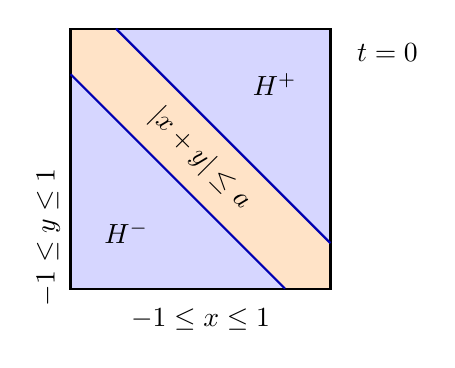
\begin{tikzpicture}[scale=1.65]
  \fill[blue!16] (-1,-1)--(.65,-1)--(-1,.65)--cycle;
  \fill[blue!16] (1,1)--(-.65,1)--(1,-.65)--cycle;
  \fill[orange!22] (-1,.65)--(.65,-1)--(1,-1)--(1,-.65)
                         --(-.65,1)--(-1,1)--cycle;
  \draw[thick] (-1,-1) rectangle (1,1);
  \draw[thick,blue!70!black] (-1,.65)--(.65,-1);
  \draw[thick,blue!70!black] (-.65,1)--(1,-.65);
  \node at (-.57,-.57) {$H^-$};
  \node at (.57,.57) {$H^+$};
  \node[fill=orange!22,inner sep=1.5pt,rotate=-45] at (0,0)
    {$|x+y|\le a$};
  \node[anchor=north] at (0,-1.08) {$-1\le x\le1$};
  \node[anchor=east,rotate=90] at (-1.17,0) {$-1\le y\le1$};
  \node[anchor=west] at (1.13,.82) {$t=0$};
 \end{tikzpicture}
 \caption{The beam sections at height zero, in parameter coordinates
 $(x,y)$, drawn with $a=0.35$. Their sloping sides satisfy
 $x+y=-a$ and $x+y=a$. The shaded closed band contains all points
 outside these two triangles. This value of $a$ illustrates the
 geometry only; the strict cost comparison will require smaller $a$.}
 \label{beam:midsection}
\end{figure}

\begin{lemma}\label{beam:finite-beams}
For fixed $a\in(0,1/2)$, partition $[0,1]$ into $k$ equal closed
intervals and choose a tag $p_I$ in each interval. The two beams admit
a covering by $2k$ cylinders with nondegenerate compact triangular
perpendicular bases, with axes parallel to $(\beta v(p_I),1)$ and
$(-\beta v(p_I),1)$, respectively. Their total normalized cost converges,
as $k\to\infty$, to
\begin{equation}\label{beam:C1}
 C_1=R_a^2\int_0^1 g(v(p))\,dp.
\end{equation}
In particular, for every $\eta>0$ a finite covering has cost at most
$C_1+\eta$.
\end{lemma}
\begin{proof}
We check the radial theorem in the physical horizontal plane, so its
area factor includes the scaling of both horizontal coordinates.
Take $e=(0,0,1)$, $p_0=(-\beta,-\beta,0)$ and
\[
 \mathbf a=(0,\beta,0),\qquad
 \mathbf b=(\beta,-\beta,0),\qquad
 \mathbf w(p)=(\beta v_1(p),\beta v_2(p),0).
\]
Then $\mathbf a+p\mathbf b=\beta(p,1-p,0)$ and
\[
 H^-=\{p_0+h(\mathbf a+p\mathbf b)+t(e+\mathbf w(p)):
       0\le p\le1,\ 0\le h\le R_a,\ |t|\le1\}.
\]
The hypotheses of Theorem~\ref{thm:radial} hold with constant cap $R_a$,
axial bound $1$ and
\[
 \mathbf w'(p)=-2aR_a(\mathbf a+p\mathbf b),\qquad
 |\det(\mathbf a,\mathbf b)|=\beta^2=\frac12,
 \qquad |\mathbf w(p)|^2=\beta^2|v(p)|^2.
\]
Consequently its one-beam limiting area is exactly
\begin{equation}\label{beam:physical-radial-cost}
 \frac{R_a^2}{4}\int_0^1\frac{dp}{\sqrt{1+\beta^2|v(p)|^2}}.
\end{equation}
For completeness, the explicit triangles in that theorem have
$A=2aR_a$, $B=aR_a$, $C=2(A+B)+1=6aR_a+1$. If $\delta=1/k$, their
individual perpendicular areas are
\[
 \frac{\delta\,[R_a+(A+C)\delta]^2}
      {4\sqrt{1+\beta^2|v(p_I)|^2}}.
\]
The orthogonal map $(X,Y,T)\mapsto(-X,-Y,T)$ gives the $k$ cylinders
for $H^+$ with the same areas. Adding the two costs and dividing by
$\beta^2/\sqrt2$ gives \eqref{beam:C1}.
\end{proof}

\subsection{The points left between the beams}

At $t=0$, the missed set is the diagonal band $|x+y|<a$ shown in
Figure~\ref{beam:midsection}. At other heights we enclose the missed
set in a tilted band with a uniform cubic error, using the transverse
coordinate $s$ and the coordinate $l$ along the diagonal:
\[
 s=x+y,\qquad l=(x-y)/2,\qquad f(t)=2at-2a^2t^3.
\]
For a constant $M>0$, to be chosen uniformly in the next lemma, define
\begin{align}
 W(t)&=\bigl(a(1-2t^2)
       +a^2t^2\{1+(1-|t|)^2+t^2\}+Ma^3\bigr)_+,
       \label{beam:width}\\
 G&=\{P(x,y,t)\in K:|s+f(t)l|\le W(t)\},\notag
\end{align}
where $q_+=\max(q,0)$.

\begin{lemma}\label{beam:coverage}
With $M=25$ in \eqref{beam:width}, one has
$K\subset H^-\cup H^+\cup G$ for every $0<a<1/2$.
\end{lemma}
\begin{proof}
Consider an interior point of $K$ outside both beams. Put
$U=x+1-t>0$ and $Y=y+1+t>0$. The strictly decreasing function
$U/p-Y/(1-p)$ runs from $+\infty$ to $-\infty$ on $(0,1)$, so there
is a $p$ satisfying
\[
 \frac Up-\frac Y{1-p}=-aR_a t,\qquad
 h=\frac Up+aR_a tp=\frac Y{1-p}-aR_a t(1-p).
\]
One of these expressions makes $h>0$ immediate, according to the sign of
$t$. They give exactly $P(x,y,t)=P(c+h r(p)+t v(p),t)$.
Because the point is outside $H^-$, necessarily $h>R_a$. Applying the same
argument to $(-x,-y,t)$ gives the corresponding reflected parameters,
also with radial parameter greater than $R_a$.

For the first representation put $d=h-R_a>0$, $q=2p-1$, and $b=R_a q/2$.
Direct substitution gives
\begin{equation}\label{beam:exact-gap}
 \begin{aligned}
 s&=-a-2atb+d,\\
 l&=t+b+dq/2-atQ,\qquad Q=R_a/4+b^2/R_a.
 \end{aligned}
\end{equation}
The reflected representation obeys these same identities with
$(-s,-l)$ in place of $(s,l)$. Since $|b|\le R_a/2<1$, the first identity
and its reflected version imply $|s|\le3a$, and then $0<d\le6a$.
Moreover $|l|\le1$ on $K$ and $Q\le R_a/2\le1$, so the second identity
gives the uniform estimate
\begin{equation}\label{beam:b-error}
 |b-(l-t)|\le4a.
\end{equation}
These bounds hold also for the reflected parameters. Since $R_a\ge3/2$
and $|l-t|\le2$, they give the numerical estimate
\begin{equation}\label{beam:uniform-constant}
 \left|Q-\frac{1+(l-t)^2}{2}\right|
 \le \frac a4+\frac{a b^2}{2R_a}
       +\frac{|b-(l-t)|\,|b+(l-t)|}{2}
 \le\left(\frac14+\frac13+6\right)a<10a.
\end{equation}
The bound is uniform, including for points tending to the boundary.

Combining the two equations in \eqref{beam:exact-gap} leaves a favorable
radial term:
\[
 s+2atl=-a+2at^2-2a^2t^2Q+d(1+atq)
 \ge -a+2at^2-a^2t^2\{1+(l-t)^2\}-20a^3,
\]
since $1+atq>0$. Reflection gives the complementary inequality
\[
 s+2atl\le a-2at^2+a^2t^2\{1+(l+t)^2\}+20a^3.
\]
Subtracting $2a^2t^3l$ from both inequalities cancels their mixed
quadratic terms, yielding
\begin{equation}\label{beam:central-strip}
 |s+f(t)l|\le a(1-2t^2)+a^2t^2(1+l^2+t^2)+20a^3.
\end{equation}
Finally the two coordinate bounds for $K$, applied to
$x=s/2+l$ and $y=s/2-l$, give
\[
 |l|\le1-|t|+|s|/2\le1-|t|+3a/2.
\]
Squaring shows $l^2\le(1-|t|)^2+3a+9a^2/4$.
Replacing $l^2$ by $(1-|t|)^2$ therefore adds at most
$(3+9a/4)a^3<5a^3$. Thus $M=25$ bounds the right side of
\eqref{beam:central-strip} by the expression inside the positive part in
\eqref{beam:width}. For such a point that expression is nonnegative,
so the point lies in $G$. We have proved coverage of the interior.
Both beams are compact, and $G$ is closed in the compact set $K$ because
$f$ and $W$ are continuous. Their finite union is closed and hence
contains the closure of the interior, namely all of $K$.
\end{proof}

\subsection{Finite horizontal cylinders for the strip}

The two beams now cover every point outside $G$. It remains to give
$G$ a finite covering whose cost can be combined with the beam cost.
\begin{lemma}\label{beam:finite-strip}
Fix $M$ as in Lemma~\ref{beam:coverage}. For every fixed $a\in(0,1/2)$
and $\eta>0$, the strip $G$ has a finite covering by cylinders with
compact rectangular perpendicular bases and normalized cost at most
$C_2+\eta$, where
\begin{equation}\label{beam:C2}
 C_2=2\sqrt{2}\int_{-1}^{1}
       \frac{W(t)}{\sqrt{1+(at-a^2t^3)^2}}\,dt.
\end{equation}
\end{lemma}
\begin{proof}
We construct the perpendicular rectangles explicitly. Define
$w(t)=(1+f(t)/2,1-f(t)/2)$, so that $s+f(t)l=w(t)\cdot(x,y)$.
Partition $[-1,1]$ into finitely many closed intervals $J$, choose
$t_J\in J$, and put
\[
 w_J=w(t_J),\quad n_J=(w_J/|w_J|,0),\quad
 A_J=\frac{\beta}{|w_J|}
 \left(\max_{t\in J}W(t)+3\max_{t\in J}|w(t)-w_J|\right).
\]
Choose a horizontal unit axis $u_J$ perpendicular to $n_J$. In its
perpendicular plane take the compact rectangle
\[
 B_J=\{z n_J+t(0,0,1): |z|\le A_J,\ t\in J\}.
\]
For a point of $G$ at height $t\in J$, its coordinate along $n_J$ is
$\beta w_J\cdot(x,y)/|w_J|$. Since $|(x,y)|\le3$ on $K$, its absolute
value is at most $A_J$. Thus $B_J+\mathbb R u_J$ covers that point.

The exact area of $B_J$ is $2A_J|J|$. Uniform continuity of $W$ and $w$
shows, as the mesh tends to zero, that the sum of these areas tends to
$\int_{-1}^{1}2\beta W(t)/|w(t)|\,dt$. Dividing by the cost unit in
\eqref{beam:normalization} and using
$|w(t)|=\sqrt{2}\sqrt{1+(at-a^2t^3)^2}$ gives
\eqref{beam:C2}. The freezing error tends to zero uniformly, including
at heights where $W$ vanishes. A sufficiently fine finite partition
therefore proves the asserted cost bound.
\end{proof}

\subsection{The strict saving survives finite approximation}\label{beam:cost-comparison}

\begin{proposition}[Cost of the shortened-beam construction]
\label{beam:counterexample}
For $a\in(0,1/2)$, fix $M=25$ in \eqref{beam:width} and put
$C(a)=C_1+C_2$, with $C_1,C_2$ as in
\eqref{beam:C1} and \eqref{beam:C2}.
For every $\zeta>0$, the tetrahedron $K$ has a finite cylinder cover
of normalized cost at most $C(a)+\zeta$, consisting of cylinders with
nondegenerate compact triangular perpendicular bases covering
$H^-\cup H^+$ and cylinders with horizontal axes and compact
rectangular perpendicular bases covering $G$.
Moreover,
\begin{equation}\label{beam:strict-gain}
 C(a)=4-\left(\frac{\sqrt2}{2}-\frac{19}{30}\right)a^2+O(a^3)
 \qquad(a\downarrow0).
\end{equation}
In particular, sufficiently small $a>0$ permits a finite cover whose
actual total base area is strictly below $A_{\min}(K)/2$.
\end{proposition}
\begin{proof}
For fixed $a$, choose the covers in Lemmas~\ref{beam:finite-beams}
and~\ref{beam:finite-strip} with excess costs at most $\zeta/2$ each.
Lemma~\ref{beam:coverage} shows that together they cover $K$, proving
the finite-cost bound. It remains to compute its limiting margin.

We now let $a\downarrow0$, keeping $M$ fixed. Write
$S_p=p^2+(1-p)^2$ and $T_p=p^4+(1-p)^4$. Uniformly in $p\in[0,1]$,
\begin{align*}
 g(v(p))
 &=\left(1-\frac{aR_a}{2}S_p+\frac{a^2R_a^2}{4}T_p\right)^{-1/2}\\
 &=1+\frac{aR_a}{4}S_p
      +a^2R_a^2\left(-\frac18T_p+\frac{3}{32}S_p^2\right)+O(a^3).
\end{align*}
The three needed integrals are
$\int_0^1S_p\,dp=2/3$, $\int_0^1T_p\,dp=2/5$, and
$\int_0^1S_p^2\,dp=7/15$. Hence
\begin{equation}\label{beam:C1-expansion}
 C_1=R_a^2+\frac{aR_a^3}{6}-\frac{a^2R_a^4}{160}+O(a^3)
     =4-\frac83a-\frac{11}{10}a^2+O(a^3).
\end{equation}
For $C_2$, its denominator is $1+O(a^2)$ and $W=O(a)$, so replacing
the denominator by $1$ changes the result by $O(a^3)$. Removing $Ma^3$
inside the positive part also has that error, because the positive-part
map is $1$-Lipschitz. Set $R=1/\sqrt{2}$. The leading expression
$a(1-2t^2)$ is positive exactly on $(-R,R)$. The quadratic perturbation
can change its sign only where $|1-2t^2|=O(a)$, a set of length $O(a)$
around the two simple zeros. On that set the integrand is $O(a^2)$.
It follows that
\begin{align}
 C_2
 &=4\sqrt{2}\int_0^R
     \left[a(1-2t^2)+a^2t^2\{1+(1-t)^2+t^2\}\right]dt+O(a^3)
       \notag\\
 &=\frac83a+\left(\frac{26}{15}-\frac{\sqrt{2}}2\right)a^2+O(a^3).
       \label{beam:C2-expansion}
\end{align}
Combining \eqref{beam:C1-expansion} and \eqref{beam:C2-expansion}
proves \eqref{beam:strict-gain}. The linear terms cancel, and the
quadratic coefficient is negative because $361/900<1/2$.
Hence $C(a)<4$ for all sufficiently small positive $a$.

To obtain a strict finite cover, first fix one such $a\in(0,1/2)$ and set
$\Delta=4-C_1-C_2>0$. Next choose the triangular beam covering of Lemma~\ref{beam:finite-beams}
and the rectangular strip covering, with excess costs each less than
$\Delta/3$. Together they cover $K$,
use unit axis directions and compact measurable perpendicular bases,
and have normalized cost less than $4$. By
\eqref{beam:normalization}, their actual total base area is less than
$4\beta^2/\sqrt{2}=\sqrt{2}=A_{\min}(K)/2$.
The parameter order is thus to fix $M=25$, then a sufficiently small
positive $a$, and finally the two finite partitions. The finite errors
use only a portion of the strict saving. The similarity described at
the start of the section transports this triangle-and-rectangle cover
to every regular tetrahedron of positive edge length.
\end{proof}

\appendix
\section{Projection areas and longest chords of simplices}
\label{sec:projections}

The main constructions use the direct projection calculation in
Section~\ref{sec:tetrahedron}. This appendix gives a more general
normalization and two alternative geometric explanations of the regular
tetrahedron's minimum shadow. They also fix the Euclidean metric for the
coordinate changes in Appendix~\ref{sec:coordinate-realizations}.

The simplex chord--projection identity below is attributed to Martini and
Weissbach \cite{MartiniWeissbach1992} by Heinrich, who states the exact
constant \cite[p.~8268]{Heinrich2014}. Martini characterizes simplices
among convex polytopes in dimension at least three by the independence
of the chord--projection product from direction
\cite[Theorem~2(C)]{Martini1991}. We compute the constant directly.

\begin{proposition}[Simplex chord--projection identity]
\label{prop:simplex}
Let $S\subset\R^d$, $d\ge2$, be a full-dimensional simplex, and let
$u\in\R^d$ be a unit vector. Write $V$ for its $d$-dimensional volume,
$A(u)$ for the $(d-1)$-dimensional volume of its orthogonal projection
onto $u^\perp$, and $L(u)$ for the greatest length of a chord of $S$
parallel to $u$. Then
\[
 A(u)L(u)=dV,\qquad
 \min_{\norm{u}=1}A(u)=\frac{dV}{\operatorname{diam}S}.
\]
\end{proposition}
\begin{proof}
Let $\lambda_0,\ldots,\lambda_d$ be the affine barycentric coordinates
of $S$, and put $b_i=\partial_u\lambda_i$. They satisfy
$\sum_i b_i=0$ and are not all zero, because the barycentric coordinate
map is injective. Hence
\[
 c=\sum_i\max(0,-b_i)=\sum_i\max(0,b_i)>0.
\]
For $s\ge0$, both $x$ and $x+su$ belong to $S$ exactly when
\[
 \lambda_i(x)\ge s\max(0,-b_i)\quad(0\le i\le d),
 \qquad \sum_i\lambda_i(x)=1.
\]
For $0\le s<1/c$, this intersection is a translate of $(1-sc)S$;
at $s=1/c$ it is one point, and above that value it is empty.
In particular, $L(u)=1/c$.

A fiber of $S$ parallel to $u$ contains two points separated by $su$
if and only if its length is at least $s$. Thus, for $0<s<L(u)$,
the projection of $S\cap(S-su)$ is the superlevel set of the fiber
length at $s$, and its $(d-1)$-volume is
$A(u)(1-s/L(u))^{d-1}$. Integrating the fiber lengths gives
\[
 V=A(u)\int_0^{L(u)}(1-s/L(u))^{d-1}\,ds
   =\frac{A(u)L(u)}{d}.
\]
This is the layer-cake formula, obtained directly by integrating
$\ell=\int_0^\infty\mathbf1_{\{s<\ell\}}\,ds$ on each fiber.
Finally, the largest chord length over all directions is the diameter:
every chord joins two points of $S$, and a pair of points realizing
the diameter is itself a chord. Taking the minimum of $dV/L(u)$
proves the second formula.
\end{proof}

\label{par:entering-faces}
There is a short alternative proof of the same constant using the
faces through which the fibers enter. If the facet opposite vertex $i$
has $(d-1)$-volume $S_i$ and altitude $h_i$, then
$V=S_i h_i/d$ and $\norm{\nabla\lambda_i}=1/h_i=S_i/(dV)$.
The facets with $b_i>0$ are the entering facets for direction $u$.
Their projections partition the shadow apart from a null set, and
facet $i$ contributes
\[
 S_i\frac{b_i}{\norm{\nabla\lambda_i}}=dVb_i.
\]
Consequently $A(u)=dV\sum_{b_i>0}b_i=dVc=dV/L(u)$.
This proof also includes directions parallel to a facet, whose
contribution is zero.

For any simplex, the distance between two convex combinations of its
vertices is at most the largest distance between two vertices. Hence the
diameter of a regular tetrahedron is its edge length. For edge length
$\ell>0$, the volume is
$\ell^3/(6\sqrt2)$ and the diameter is $\ell$. Therefore
\begin{equation}\label{eq:regular-normalization}
 A_{\min}=\frac{\ell^2}{2\sqrt2},\qquad
 \frac{A_{\min}}2=\frac{\ell^2}{4\sqrt2}.
\end{equation}
For example, the volume follows by taking a face of area
$\sqrt3\ell^2/4$ and altitude $\sqrt{2/3}\ell$.
A similarity of ratio $r>0$ multiplies every perpendicular base area
and $A_{\min}$ by $r^2$, while preserving all cylinder counts and
both normalized covering costs.

\subsection{A different reason that an edge direction minimizes the shadow}

The chord identity is not needed to locate the minimum for a regular
tetrahedron. There is an independent argument based on the piecewise
linear expression in Cauchy's face formula~\eqref{eq:cauchy}.
Indeed, some minimizing direction for any tetrahedron is parallel to an
edge; for a regular tetrahedron all edge directions give the same area.
To see this directly, argue as follows.
The continuous positive projection-area function $A$ attains its
minimum on the unit sphere. Suppose that a minimizing $u$ is
perpendicular to at most one facet normal. Choose a unit $v\perp u$,
also perpendicular to that normal if it exists. For sufficiently small
$\theta>0$, all nonzero signs in the face formula stay unchanged at
\[
 u_\pm=(\cos\theta)u\pm(\sin\theta)v,
\]
and a zero scalar product remains zero. Consequently
\[
 A(u_+)+A(u_-)=2\cos\theta\,A(u)<2A(u),
\]
contradicting minimality. Equivalently, along this great-circle arc the
area is a fixed linear form and satisfies $A''=-A<0$, so it cannot
have a local minimum. A minimizing direction is therefore perpendicular
to at least two facet normals and hence parallel to the common edge.
For a regular tetrahedron, isometries permute the edges. In the edge-$2$
model
\[
 \{(x,y,\sqrt2 t):0\le t\le1,\ |x|\le t,\ |y|\le1-t\},
\]
projection in the $x$-direction has area
$\sqrt2\int_0^1 2(1-t)\,dt=\sqrt2$. Scaling gives
$\ell^2/(2\sqrt2)$ for every edge direction.

\paragraph{The regular normal frame.}
A further algebraic check, useful in barycentric coordinates, comes
from the regular tetrahedron's normal frame.\label{par:normal-frame}
If its outward unit
normals are $n_1,\ldots,n_4$, then
\[
 \sum_i n_i=0,\qquad \sum_i n_i n_i^{\mathsf T}=\frac43 I.
\]
These identities follow, for example, from the four vectors
$(1,1,1),(1,-1,-1),(-1,1,-1),(-1,-1,1)$ after normalization.
For a unit direction $u$, set $s_i=n_i\cdot u$ and let $P$ be the
sum of their positive values. The negative values have absolute sum
$P$, so
\[
 \frac43=\sum_i s_i^2\le2P^2.
\]
Since a facet has area $\sqrt3\ell^2/4$, the positive-face form of
Cauchy's formula gives
$A(u)=(\sqrt3\ell^2/4)P\ge\ell^2/(2\sqrt2)$.
In the barycentric realization\label{par:barycentric-projection}
$\{(a,b,c,d)\in[0,\infty)^4:a+b+c+d=1\}$, the Euclidean
metric is the one induced from $\R^4$, the edge length is $\sqrt2$,
and the same calculation reads
$A(u)=\tfrac12\sum_i|u_i|\ge1/\sqrt2$ for unit sum-zero vectors $u$.
These equivalent frame calculations fix the metric explicitly when
we change coordinates below.

\section{Radial caps and their overlap margins}
\label{sec:cap-choices}

The overlapping construction in Section~\ref{sec:tetrahedron} used a
cubic addition to a quadratic radial cap. This appendix describes other
caps that preserve coverage and strict saving. A common criterion proves
all of them first. The subsequent identities give alternative proofs and
coordinate forms, useful when a cap is specified by its square or by a
fractional power of the tilt.

Keep the tetrahedron \eqref{eq:tetrahedron}, the functions $G,H,D_0$,
and the upper and lower parametrizations \eqref{eq:upper-sweep} and
\eqref{eq:lower-sweep}. In this appendix replace their common cap by a
continuous nonnegative function $R_\eps$ on $[-1,1]$. Write
\begin{equation}\label{eq:general-cap-cost}
 Q_R(\eps)=\int_{-1}^1
 \frac{R_\eps(r)^2}{2\sqrt{1+\eps^2D_0(r)}}\,dr.
\end{equation}
Whenever the two sweeps cover $K$, Theorem~\ref{thm:radial} gives
$2N$ triangular-base cylinders, for each $N\ge1$, whose total areas
converge to $2hQ_R(\eps)$ as the mesh tends to zero. The actual swept
projections have the same limiting total area by Theorem~\ref{thm:radial},
although their finite areas can differ from the triangular areas. The tilt
is held fixed throughout the refinement.

\subsection{A common criterion and the exact cost}

\begin{proposition}[Four radial cap choices]\label{prop:cap-choices}
For the tetrahedron and paired sweeps just described, each of the
following caps gives coverage for every sufficiently small $\eps>0$:
\begin{align*}
 R_\eps(r)&=1+\eps^2(H(r)+\beta), &&\beta>0,\tag{L}\\
 R_\eps(r)&=1+\eps^2H(r)+c\eps^3, &&c\ge9/2,\tag{C}\\
 R_\eps(r)&=1+\eps^2H(r)+c\eps^{5/2}, &&c>0,\tag{F}\\
 R_\eps(r)&=\sqrt{1+2\eps^2(H(r)+\beta)},&&\beta>0.\tag{S}
\end{align*}
For (C), coverage in fact holds for every $\eps>0$.
Their normalized costs have the respective expansions
\begin{align}
 Q_R(\eps)&=1+(2\beta-1/30)\eps^2+O(\eps^4), &&\text{(L), (S)},
 \label{eq:fixed-cap-cost}\\
 Q_R(\eps)&=1-\eps^2/30+2c\eps^3+O(\eps^4), &&\text{(C)},
 \label{eq:cubic-cap-cost}\\
 Q_R(\eps)&=1-\eps^2/30+2c\eps^{5/2}+O(\eps^4), &&\text{(F)}.
 \label{eq:fractional-cap-cost}
\end{align}
Thus (L) and (S) give strict saving when $0<\beta<1/60$;
(C) and (F) give strict saving for every stated fixed $c$.
In each case one first fixes a tilt giving coverage and strict saving,
and then chooses a finite sufficiently fine partition.
\end{proposition}
\begin{proof}
The root selection in Proposition~\ref{prop:coverage} is independent
of the cap. Suppose first that
$R_\eps(r)=1+\eps^2(H(r)+b_\eps(r))$, where $b_\eps\ge0$.
If both caps fail, the estimates through \eqref{eq:interface-error}
and the ensuing exact identity apply without change: only nonnegativity
of the cap correction was used there. They give
\begin{equation}\label{eq:cap-failure-bound}
 \frac{xq-yp}{\eps}\le H(p)+H(q)+9\eps.
\end{equation}
The failed caps require the left side to exceed
$H(p)+H(q)+b_\eps(p)+b_\eps(q)$. Consequently
\begin{equation}\label{eq:padding-criterion}
 b_\eps(p)+b_\eps(q)\ge9\eps\quad(p,q\in[-1,1])
\end{equation}
is a sufficient coverage condition. Taking $b_\eps=\beta$, $c\eps$,
or $c\sqrt\eps$ proves (L), (C), and (F), with the stated ranges.
The strict inequality furnished by failure permits equality in
\eqref{eq:padding-criterion}.

For (S), put $A=H+\beta$. Rationalizing the square root gives the
exact expression
\[
 R_\eps=1+\eps^2\left(A-
 \frac{2\eps^2A^2}{(\sqrt{1+2\eps^2A}+1)^2}\right).
\]
Since $A$ is bounded and $\beta>0$, its effective padding is at least
$\beta/2$ for all sufficiently small $\eps$. Condition
\eqref{eq:padding-criterion} again applies. In particular the square-root
cap has not been replaced by its Taylor polynomial.

The cost calculation is uniform in $r$. For (L) and (S), respectively,
\[
 R_\eps^2=1+2\eps^2(H+\beta)+O(\eps^4),
 \qquad R_\eps^2=1+2\eps^2(H+\beta).
\]
For (C) or (F), with $\gamma=3$ or $5/2$,
$R_\eps^2=1+2\eps^2H+2c\eps^\gamma+O(\eps^4)$.
Multiply by
$(1+\eps^2D_0)^{-1/2}=1-\eps^2D_0/2+O(\eps^4)$,
divide by two, and integrate. The integrals already evaluated in
Section~\ref{sec:tetrahedron} give
$\int(H-D_0/4)=-1/30$. This proves all three expansions.
For (L) and (S) with $0<\beta<1/60$, and for (C) and (F) with every
stated $c$, the negative quadratic term dominates the higher-order terms.
Fixing such a tilt and then refining the partition gives the finite saving.
\end{proof}

For reference, the following rational fixed margins all give strict
saving. Several appear in the explicit feet and coordinate realizations
of Appendices~\ref{sec:finite-footprints}--\ref{sec:coordinate-realizations}.
Their exact quadratic cost coefficients are
\begin{center}
\begin{tabular}{c|rrrrrrr}
$\beta$&$1/120$&$1/125$&$1/500$&$4/625$&$1/100$&$1/200$&$1/250$\\
\hline
$2\beta-1/30$&$-1/60$&$-13/750$&$-11/375$&$-77/3750$&$-1/75$&$-7/300$&$-19/750$
\end{tabular}
\end{center}
The square-root choices $\beta=1/120,1/125$ have the same displayed
quadratic coefficients as their linear counterparts, but their caps and
finite covers are different. Cubic choices $c=5,12,20,64$ contribute,
respectively, $10,24,40,128$ at order $\eps^3$. Fractional choices
$c=1,4\sqrt2,8\sqrt2$ contribute $2,8\sqrt2,16\sqrt2$ at order
$\eps^{5/2}$. Each constant here specifies an actual cap rather than an
identification based only on a leading coefficient.

\subsection{Alternative identities for the overlap}

The coverage and saving for all four caps have now been proved.
The following arguments are alternatives to the common criterion, not
additional requirements. The first uses the monotonicity of $G$ in the
squared angular variable; the second keeps positive weights on the radial
parameters; the third avoids expanding a square-root cap.

\paragraph{Fixed margins and monotone polynomials.}
For the roots in \eqref{eq:root-one}--\eqref{eq:root-two}, the segment
equations are
\[
 y=\rho q-\eps xG(q),\qquad
 x=\sigma p+\eps yG(p),\qquad
 \rho+\sigma=2+\eps(xq-yp).
\]
Under joint cap failure for (L), $\rho,\sigma>1$. Put
$E=\rho+\sigma-2$. Since $|\rho-\sigma|\le E$, substitution gives
\[
 E=\eps(\sigma-\rho)pq+\eps^2\{yqG(p)+xpG(q)\}.
\]
All variables except the radial parameters are bounded independently of
$\eps$. Absorbing $\eps E$ for $\eps<1/2$ shows $E=O(\eps^2)$.
Thus $\rho,\sigma=1+O(\eps^2)$ and $x=p+O(\eps)$,
$y=q+O(\eps)$. A further substitution gives uniformly
\[
 E=\eps^2\{q^2G(p)+p^2G(q)\}+O(\eps^3)
 \le\eps^2(H(p)+H(q))+O(\eps^3),
\]
because
$(p^2-q^2)(G(p)-G(q))=(p^2-q^2)^2/2\ge0$.
The failed caps instead give
$E>\eps^2(H(p)+H(q)+2\beta)$, a contradiction for small $\eps$.
Equivalently, one can argue by compactness without estimating the
uniform cubic constant. If failure occurred along $\eps\downarrow0$,
a subsequence would have $p\to P$, $q\to Q$, $x\to P$, $y\to Q$,
and $t/\eps\to PQ$, by the same root equations and cap inequalities.
The exact identity in the proof of Proposition~\ref{prop:coverage} gives
\[
 \lim\frac{xq-yp}{\eps}=(P^2+Q^2)/2+P^2Q^2.
\]
The required lower limit $H(P)+H(Q)+2\beta$ exceeds this by
$(P^2-Q^2)^2/2+2\beta>0$. This establishes the fixed-margin
coverage directly, including all boundary points through the root lemma.

\paragraph{Positive weighted sums and fractional margins.}
The preceding segment equations also give the exact identity
\begin{equation}\label{eq:weighted-radial-identity}
 (1+\eps pq)\rho+(1-\eps pq)\sigma
 =2+\eps^2\{qG(p)y+pG(q)x\}.
\end{equation}
Under failure for (F), the inequalities $\rho,\sigma>1$ imply
$x=p+O(\eps)$ and $y=q+O(\eps)$, uniformly. Thus its right side is
at most $2+\eps^2(H(p)+H(q))+O(\eps^3)$. For $\eps<1$ both
weights on the left are positive. Substituting the two failed caps makes
that side strictly greater than
\[
 2+\eps^2(H(p)+H(q))+2c\eps^{5/2}+O(\eps^3).
\]
The positive fractional term dominates the cubic error. This proves
coverage by a weighted cancellation, without discarding the fractional
term from the cost expansion.

There is a related complementary-coordinate identity. Put
$T=t-\eps xq=1-\rho$ and $S=-t+\eps yp=1-\sigma$. Directly from
the segment equations,
\begin{align}
 (1+\eps xq)T&=t-\eps xy-\eps^2x^2G(q),\label{eq:complementary-one}\\
 (1-\eps yp)S&=-t+\eps xy-\eps^2y^2G(p).\label{eq:complementary-two}
\end{align}
If both caps fail, then $T,S<0$. For $\eps\le1/4$ the two
coefficients are at least $1/2$. Adding the identities therefore gives
\begin{equation}\label{eq:complementary-bound}
 |T|,|S|\le16\eps^2.
\end{equation}
This bounds each missed intercept, rather than only their sum. The
segment equations give $|x-p|,|y-q|\le C\eps$ for a uniform $C$.
For cap (L), substituting the strict failures $T<-\eps^2(H(q)+\beta)$ and
$S<-\eps^2(H(p)+\beta)$ into the sum then requires
\[
 x^2G(q)+y^2G(p)>H(p)+H(q)+2\beta-O(\eps).
\]
The left side is at most $p^2G(q)+q^2G(p)+O(\eps)$ and hence at
most $H(p)+H(q)+O(\eps)$, again a contradiction. Rescaling the axial
coordinate by $t=kz$ and the tilt by $\eps=k\tau$, with
$k=1/\sqrt2$, turns \eqref{eq:complementary-bound} into the explicit
physical-intercept estimate $|T/k|,|S/k|\le16k\tau^2$.

\paragraph{Squared radial parameters.}
The same roots satisfy two further exact identities:
\begin{equation}\label{eq:squared-radial-identities}
 \rho^2=(1-t)^2+2\eps xy+\eps^2x^2,
 \qquad
 \sigma^2=(1+t)^2-2\eps xy+\eps^2y^2.
\end{equation}
For example, expand $(1-t+\eps xq)^2$ and substitute
$2xy=2(1-t)xq+\eps x^2(q^2-1)$ from the first root equation.
For the square-root cap (S), joint failure requires
\[
 2(t/\eps)^2+x^2+y^2>2H(p)+2H(q)+4\beta.
\]
Along any hypothetical sequence of failures approaching zero tilt,
the root and cap inequalities give $x\to P$, $y\to Q$ and
$t/\eps\to PQ$. The limiting right side exceeds the left by
$(P^2-Q^2)^2+4\beta$, a contradiction. For (L), the square of its
cap is at least $1+2\eps^2(H+\beta)$, so the same argument applies.
This retains both the square-root construction and the square-identity
proof for a polynomial cap.


\paragraph{A larger cubic certificate.}
For the cubic choice $c=12$, suppose both selected radial parameters
exceed their caps. The root estimates in Proposition~\ref{prop:coverage}
give
\[
 0<\rho-1,\sigma-1\le\rho+\sigma-2
 =\eps\{(x-p)q-(y-q)p\}\le6\eps^2\le12\eps^2.
\]
Their difference obeys the same bound. Multiplying \eqref{eq:cap-failure-bound} by $\eps^2$ gives an
error $9\eps^3$, which is bounded by the combined padding
$24\eps^3$. Thus this choice also provides a cubic certificate
with that larger constant. Its total limiting cost is
$2\sqrt2(1-\eps^2/30+24\eps^3+O(\eps^4))$.

\subsection{A quantitative complementary calculation at half height}

An exact weighted calculation gives another explicit cubic certificate.
Use coordinates $(X,Y,Z)$ with
$|X|\le1-Z$, $|Y|\le Z$, and their physical realization
$(X/2,Y/2,Z/\sqrt2)$. For $r\in[-1,1]$ define
\[
 \alpha(r)=(1+r^2)/4,\quad \beta(r)=r/2,\quad
 F(r)=r^2(1+r^2)/16.
\]
The two line families are
\begin{align*}
 Y&=ur+\delta X\alpha(r),& Z&=u+\delta X\beta(r),\\
 X&=vs-\delta Y\alpha(s),&1-Z&=v-\delta Y\beta(s).
\end{align*}
The crossing lemma supplies $u,v\ge0$. Both families use the cap
$R_\delta(r)=1/2+\delta^2F(r)+4\delta^3$.
Their exact complementary identity is
\begin{equation}\label{eq:half-height-compensation}
 (u-1/2)(1-\delta Xr)+(v-1/2)(1+\delta Ys)
 =\delta^2\{X^2\alpha(r)+Y^2\alpha(s)\}.
\end{equation}
To verify it, expand
$Z-\delta XY=1/2+(u-1/2)(1-\delta Xr)-\delta^2X^2\alpha(r)$
and its complementary equation, and add.

Suppose both caps fail and $0<\delta\le1/2$. The weights in
\eqref{eq:half-height-compensation} are at least $1/2$, since
$|X|,|Y|\le1$. Its right side is at most $\delta^2$, so each
positive radial excess is at most $2\delta^2$. It follows that
$|Y-r/2|,|X-s/2|\le2\delta^2+\delta/2\le3\delta/2$. Therefore
\[
 X^2\alpha(r)+Y^2\alpha(s)
 \le\frac{s^2\alpha(r)+r^2\alpha(s)}4+\frac94\delta
 \le F(r)+F(s)+\frac94\delta.
\]
Here $|X+s/2|,|Y+r/2|\le3/2$, $\alpha\le1/2$, and the last
inequality is monotonicity in $r^2,s^2$. Failed caps, however, make
\eqref{eq:half-height-compensation} divided by $\delta^2$ exceed
\[
 (1-\delta)(F(r)+F(s)+8\delta)
 \ge F(r)+F(s)+\frac{15}{4}\delta,
\]
because $F\le1/8$. The incompatible constants $9/4$ and $15/4$
prove coverage throughout $0<\delta\le1/2$.

Replacing $4\delta^3$ by $\delta^{5/2}$ gives a second useful
version for all sufficiently small positive $\delta$. To see the fractional cancellation directly, set $a=1/2$,
$P(\xi)=a/2+\xi^2/(2a)$ and $g(\xi)=\xi^2P(\xi)$.
The identity before \eqref{eq:half-height-compensation} becomes
\[
 Z=a+\delta XY-\delta^2P(ar)X^2
       +(u-a)(1-\delta rX).
\]
With both caps failed, $|Y-ar|,|X-as|=O(\delta)$ uniformly and the
positive factors are bounded away from zero. Bounded derivatives of
$P,g$ consequently give
\begin{align*}
 Z&>a+\delta XY+\delta^2(g(Y)-P(Y)X^2)
       +\delta^{5/2}-C\delta^3,\\
 Z&<a+\delta XY-\delta^2(g(X)-P(X)Y^2)
       -\delta^{5/2}+C\delta^3.
\end{align*}
Their incompatibility follows from the exact identity
\[
 g(X)+g(Y)-P(X)Y^2-P(Y)X^2
 =\frac{(X^2-Y^2)^2}{2a}\ge0.
\]
Thus the complementary and the positive-weight arguments both preserve
fractional padding with its proper, non-fourth-order leading remainder.
The affine change $x=2Y$, $y=2X$, $t=2Z-1$ takes these two
half-height families to the earlier canonical families with
$\eps=\delta/2$. The first family becomes the lower family with
radial parameter $2u$, angular parameter $r$, and free coordinate $y=2X$;
the second becomes the upper family with radial parameter $2v$, angular
parameter $s$, and free coordinate $x=2Y$. The cubic and fractional caps become, respectively,
$1+\eps^2H+64\eps^3$ and
$1+\eps^2H+8\sqrt2\eps^{5/2}$.

\section{Finite enclosures and their areas}
\label{sec:finite-footprints}

Theorem~\ref{thm:radial} supplies triangular bases and the exact limiting
cost for actual swept projections. This appendix records other finite
choices: polygonal feet with explicit area formulas, convex trapezoids,
and neighborhoods of the shortened beams' radial sectors. Each choice
keeps the same limiting cost as its sweep. Their finite areas and geometric
properties can differ, so we specify the enclosure and control its area
before taking a limit.

\subsection{One intercept identity, several enclosures}

Use a cap $R_\eps$ and fix a positive tilt for which
Appendix~\ref{sec:cap-choices} gives coverage. Retain $h=\sqrt2$.
For a closed interval $I\subset[-1,1]$ of positive length $d$, a tag $c\in I$,
and $M=\max_I R_\eps$, the upper-sweep point with parameters
$q,\rho,x$ has frozen intercept
\begin{equation}\label{eq:quadratic-foot-identity}
 u=\rho-\eps x(q-c),\qquad
 Y=qu+\frac{\eps x}{2}(q-c)^2,
 \qquad 0\le\rho\le M,\quad |x|\le2.
\end{equation}
The physical intercept point is $(0,Y,h(1-u))$. Its area element is
$h\,dY\,du$, and projection perpendicular to the frozen direction
multiplies area by $(1+\eps^2D_0(c))^{-1/2}$. The lower family is
obtained by the same orthogonal map as before.

Let $m$ be the midpoint of $I$. For positive constants $A,B$, an
absolute-value footprint is
\begin{equation}\label{eq:abs-foot-family}
 -Ad\le u\le M+Ad,\qquad
 |Y-mu|\le \frac d2|u|+Bd^2.
\end{equation}
For any tag, it contains \eqref{eq:quadratic-foot-identity} when
$A\ge2\eps$ and $B\ge\eps$. For midpoint tags, the sharper sufficient
conditions are $A\ge\eps$ and $B\ge\eps/4$.
Indeed $|q-c|\le d$ for any tag and $|q-c|\le d/2$ at the midpoint;
\eqref{eq:quadratic-foot-identity} then bounds the radial displacement
by $2\eps|q-c|$ and the extra transverse displacement by
$\eps|q-c|^2$. The angular sector itself has width $d|u|$.
The exact coordinate area is
\begin{equation}\label{eq:abs-foot-area}
 \frac{dM^2}{2}+(A+2B)Md^2+(A^2+4AB)d^3.
\end{equation}
This follows by integrating $d|u|+2Bd^2$ from $-Ad$ to $M+Ad$.
The footprint is a compact polygonal set. With a negative collar it is
generally nonconvex: the upper-boundary points at $u=\pm Ad$ have a
midpoint above the upper boundary at $u=0$.

\paragraph{The original cubic cap.}
For the cap $R_\eps=1+\eps^2H+5\eps^3$ used in
Section~\ref{sec:tetrahedron}, take $N$ equal intervals of length $d=2/N$,
midpoint $c$, and $R_I=\max_I R_\eps$. The absolute-value choice
$A=2\eps$, $B=\eps$ can be written
\begin{equation}\label{eq:polygonal-foot}
 P_I=\{(0,Y,h(1-u)):
    -2\eps d\le u\le R_I+2\eps d,\quad
    Y\in uI+[-\eps d^2,\eps d^2]\}.
\end{equation}
The intercept identity \eqref{eq:quadratic-foot-identity} proves containment.
Project $P_I$ perpendicular to $v_I=(1,-\eps G(c),h\eps c)$ and apply
$\mathcal R$ to obtain the corresponding lower-family base. These $2N$
cylinders cover the tetrahedron, and each upper base has exact area
\begin{equation}\label{eq:polygonal-area}
 \frac{h}{\sqrt{1+\eps^2D_0(c)}}
 \int_{-2\eps d}^{R_I+2\eps d}(d|u|+2\eps d^2)\,du.
\end{equation}
By \eqref{eq:abs-foot-area}, this integral is
$dR_I^2/2+O_\eps(d^2)$ uniformly over the intervals. Their total cost
therefore converges to \eqref{eq:cost-integral}. For sufficiently small
fixed $\eps$, this limit is below $2h$, so a sufficiently fine finite
partition gives a polygonal cover within the same strict area gap.
These feet are generally nonconvex;
the following affine choices give convex alternatives.

\paragraph{Affine feet.}
At a midpoint tag $c=m$ one can instead use the affine footprint
\begin{equation}\label{eq:midpoint-affine-foot}
 -Ad\le u\le M+Ad,\qquad
 |Y-cu|\le \frac d2u+Bd^2.
\end{equation}
For containment it suffices that $A\ge\eps$ and $B\ge3\eps/4$.
To check this, use the other form of the exact intercept identity,
\[
 Y-cu=(q-c)\rho-\frac{\eps x}{2}(q-c)^2.
\]
Its absolute value is at most $d\rho/2+\eps d^2/4$, and
$\rho\le u+\eps d$. These are precisely the asserted bounds.
If $B\ge A/2$, the width is nonnegative on the entire radial interval,
and the coordinate area is exactly
\begin{equation}\label{eq:affine-foot-area}
 \frac{dM^2}{2}+(A+2B)Md^2+4ABd^3.
\end{equation}
For $B>A/2$ this is a nondegenerate compact trapezoid; for
$B=A/2$ it is a nondegenerate compact triangle with its vertex at
$u=-Ad$, provided $M+2Ad>0$. All cap choices here have $M>0$.
The projection is nonsingular, so it preserves convexity and polygon type.

Freezing at a left endpoint gives another affine certificate. Put
$c=\min I$ and $W=Y-cu$. Then
\[
 W=(q-c)u+\frac{\eps x}{2}(q-c)^2.
\]
The footprint
\begin{equation}\label{eq:endpoint-affine-foot}
 -2\eps d\le u\le M+2\eps d,\qquad
 -3\eps d^2\le W\le du+3\eps d^2
\end{equation}
contains all intercepts. For $u\ge0$, the product $(q-c)u$ lies
between $0$ and $du$. For $u<0$, it lies between $du$ and $0$;
the radial bound gives $|u|d\le2\eps d^2$. The error term has
magnitude at most $\eps d^2$, proving both inequalities. This compact
convex trapezoid has area \eqref{eq:affine-foot-area} with
$A=2\eps$, $B=3\eps$.

The following choices illustrate the geometric freedom while keeping all
constants in the same physical coordinate system:
\begin{center}
\begin{tabular}{lll}
freezing tag & foot & $(A,B)$\\ \hline
arbitrary & absolute-value & $(2\eps,\eps)$\\
midpoint & absolute-value & $(\eps,\eps)$\\
midpoint & affine trapezoid & $(\eps,3\eps/4)$\\
midpoint & affine trapezoid & $(4\eps,4\eps)$\\
midpoint & affine trapezoid & $(\eps,\eps)$\\
midpoint & triangle & $(2\eps,\eps)$\\
left endpoint & affine trapezoid & $(2\eps,3\eps)$
\end{tabular}
\end{center}
For example, the midpoint trapezoid $(\eps,3\eps/4)$ is contained
in the absolute-value foot $(\eps,\eps)$ for the same cap and
interval. Their half-width difference is $\eps d^2/4$ on $u\ge0$
and $-du+\eps d^2/4$ on $u\le0$. They have the same leading
area but distinct finite areas and convexity properties.
The more generously padded choices $A=B=1$ when $\eps\le1/8$,
and $A=B=\sqrt2+2\eps$, also satisfy the absolute-value certificate.
They are useful when the original coordinate mesh is chosen independently
of the small tilt.

In all these formulas the area is $dM^2/2+O_\eps(d^2)$, uniformly
in $I$ for fixed tilt and bounded cap. Multiplication by the physical
projection factor and Riemann summation therefore give the exact total
limit $2hQ_R(\eps)$. The actual swept projections have that same limit:
the certificates give the upper bound, and the zero-free-coordinate
sectors in Theorem~\ref{thm:radial} give the matching lower bound.
This equality of limits does not identify the finite bases. For example,
freezing actual sweeps at left endpoints and projecting explicit feet at
midpoints need not give the same bases or the same finite cost.

\subsection{Two exact formulas at unit edge length}

It is useful to write two of the finite enclosures in coordinates in
which the tetrahedron has edge one. Let $h_1=1/\sqrt2$ and fix a
sufficiently small $\eta>0$. For the square-root cap
\[
 T_\eta(s)^2=\frac14+\eta^2\left(s^2/4+s^4+1/960\right),
 \qquad |s|\le\frac12,
\]
use the tetrahedron
$|x|\le(1-t)/2$, $|y|\le t/2$ in physical coordinates
$(x,y,h_1t)$. The first line family is
\[
 y=sp+\eta x(1/4+s^2),\qquad t=p+2\eta xs,
 \qquad 0\le p\le T_\eta(s),
\]
and the second exchanges $x,y$, $t,1-t$, and changes the sign of the
tilt. Under $X=4y$, $Y=4x$, $Z=2t-1$ this is cap (S) with
$\eps=\eta/2$ and $\beta=1/120$, so the coverage proof is already
complete: the first family becomes the canonical lower family with
angle $2s$ and radius $2p$; the second becomes the upper family.
For midpoint intervals of length $\Delta=1/N$, midpoint
$s_j$, and maximum $T_j$, the intercept triangles are
\begin{equation}\label{eq:unit-triangle-foot}
 -\eta\Delta\le c\le T_j+\eta\Delta,
 \qquad |b-s_jc|\le\frac\Delta2(c+\eta\Delta).
\end{equation}
Their physical area is exactly
\begin{equation}\label{eq:unit-triangle-area}
 \frac{h_1\Delta}{2}(T_j+2\eta\Delta)^2.
\end{equation}
For completeness, subtracting the frozen direction from a represented
point gives
$c=p+2\eta x(s-s_j)$ and
$b-s_jc=(s-s_j)p+\eta x(s-s_j)^2$.
Since $|x|\le1/2$,
$|c-p|\le\eta\Delta/2$ and
$|b-s_jc|\le\Delta(p+\eta\Delta/4)/2
\le\Delta(c+\eta\Delta)/2$.
Projecting these intercept triangles gives $2N$ triangular bases whose
cylinders cover for every $N\ge1$, not only after mesh refinement.
Projection divides their physical intercept area by
$\sqrt{1+\eta^2((1/4+s_j^2)^2+2s_j^2)}$.
Summing over both families gives the exact limit
\[
 h_1\int_{-1/2}^{1/2}
 \frac{1/4+\eta^2(s^2/4+s^4+1/960)}
 {\sqrt{1+\eta^2((1/4+s^2)^2+2s^2)}}\,ds
 =h_1\left(\frac14-\frac{\eta^2}{960}+O(\eta^4)\right).
\]
This is a particular triangle formula in addition to the arbitrary-tag
triangles furnished by Theorem~\ref{thm:radial}.

For the half-height construction of Appendix~\ref{sec:cap-choices}, take intervals
of half-length $\rho=1/N$, midpoint $p_j$, and maximum cap $M_j$.
Put $e=\delta\rho/2$. In its normalized intercept coordinates define
\begin{equation}\label{eq:halfheight-trapezoid}
 D_j=\{(v,w):-e\le w\le M_j+e,\quad
             |v-p_jw|\le\rho(w+2e)\}.
\end{equation}
Its exact coordinate area is
\begin{equation}\label{eq:halfheight-trapezoid-area}
 |D_j|=\rho(M_j^2+6eM_j+8e^2).
\end{equation}
An actual first-family intercept has
$(v,w)=(ur+\sigma(r+p_j)/2,u+\sigma)$ with
$\sigma=\delta X(r-p_j)/2$, so $|\sigma|\le e$ and
$|v-p_jw|\le\rho(u+e/2)\le\rho(w+2e)$.
The second-family formula has
$\sigma=-\delta Y(s-p_j)/2$ and gives the same bounds.
The perpendicular projections of these trapezoids give $2N$ compact
convex bases whose cylinders cover the tetrahedron.
The physical foot area multiplier is $h_1/2$, and its projection factor
is $(1+\delta^2(\alpha(p_j)^2+2\beta(p_j)^2))^{-1/2}$.
Consequently the cubic cap gives total area limit
\[
 \frac{h_1}{2}\int_{-1}^1
 \frac{R_\delta(r)^2}{\sqrt{1+\delta^2(\alpha(r)^2+2\beta(r)^2)}}\,dr
 =\frac{h_1}{2}\left(\frac12-\frac{\delta^2}{240}+O(\delta^3)\right).
\]
The exact cubic coefficient can also be retained by
\eqref{eq:cubic-cap-cost}. Coverage holds for $0<\delta\le1/2$;
strict saving uses a sufficiently small such $\delta$ before selecting
$N$. The count is exactly two cylinders per interval and is not asserted
to remain bounded as the tilt tends to zero.

\subsection{Beam bases from neighborhoods of two triangles}
\label{beam:neighborhood-alternative}
We finish with a different geometry for the beam bases of
Section~\ref{beam:section}. Fix $a\in(0,1/2)$ and recall
\[
 R_a=2-a,\quad c=(-1,-1),\quad r(p)=(p,1-p),\quad
 v(p)=(1,-1)+aR_a(-p^2,(1-p)^2).
\]
The physical map is $P(x,y,t)=(\beta x,\beta y,t)$ with
$\beta=1/\sqrt2$, and the first beam $H^-$ consists of
$P(c+h r(p)+t v(p),t)$ for $0\le p\le1$, $0\le h\le R_a$,
and $|t|\le1$. Its reflection in the vertical axis is the second beam.
Using the projection factor $g$ from \eqref{beam:projection-factor},
the combined limiting normalized cost is
$C_1=R_a^2\int_0^1g(v(p))\,dp$.
We construct bases from neighborhoods of two triangular sectors; their
finite areas differ from the triangular bases in the main proof.

Partition $[0,1]$ into $k$ closed intervals $I$ of length $\delta=1/k$,
and freeze the direction at each midpoint $p_I$. Sliding a point of $H^-$
to height zero along $(\beta v(p_I),1)$ leaves the planar intercept
$c+h r(p)+t(v(p)-v(p_I))$. For $e=p-p_I$, the quadratic formula for $v$
gives the exact identity
\begin{equation}\label{beam:radial-cancellation}
 v(p)-v(p_I)=-2aR_a e\,r(p)+aR_a e^2(1,-1).
\end{equation}
The first term changes only the radial parameter $h$. Indeed,
$|2aR_a et|\le\delta$ and
$|aR_a e^2t(1,-1)|\le\sqrt2\delta^2/4<\delta^2$ because
$aR_a<1$ and $|e|\le\delta/2$. Thus every intercept lies in $c+S_I$,
where $S_I$ is the closed $\delta^2$-neighborhood of
\[
 Q_I=\{d r(p):p\in I,\ -\delta\le d\le R_a+\delta\}.
\]
The set $Q_I$ consists of two triangles, with total area
\[
 |Q_I|=\frac{(R_a+\delta)^2+\delta^2}{2}\,\delta.
\]
This follows either from their vertex determinants or from the Jacobian
$|d|$ of $(d,p)\mapsto d r(p)$. Their perimeters are uniformly bounded.
For a triangle, a radius-$\rho$ neighborhood adds at most its perimeter
times $\rho$ plus $\pi\rho^2$ in area: decompose the added region
into edge rectangles and vertex sectors, whose angles sum to $2\pi$.
Applying this to both triangles,
with $\rho=\delta^2$, gives
\[
 |S_I|\le \frac{R_a^2}{2}\delta+O(\delta^2).
\]
The constant is uniform over the intervals. Projecting $P(c+S_I,0)$ onto
the perpendicular plane produces a compact base whose cylinder covers
the corresponding part of $H^-$. By \eqref{beam:projection-factor}, its normalized cost is
$|S_I|g(v(p_I))$. The unpadded sector
$\{d r(p):p\in I,\ 0\le d\le R_a\}$ lies in $Q_I\subset S_I$
and has area $R_a^2\delta/2$. Combining this lower bound with the
upper estimate gives the first beam's total normalized cost as
\[
 \frac{R_a^2}{2}\sum_I\delta\,g(v(p_I))+O_a(\delta)
 \longrightarrow \frac{C_1}{2}.
\]
Since $g\circ v$ is smooth on $[0,1]$, the midpoint sum differs from
its integral by $O_a(\delta)$. The orthogonal map
$(X,Y,T)\mapsto(-X,-Y,T)$ supplies the reflected covering at the same
cost. Thus, for every positive integer $k$, these $2k$ cylinders cover
the two beams, and their total normalized cost is
$C_1+O_a(k^{-1})$. The quadratic transverse remainder in
\eqref{beam:radial-cancellation} makes the summed padding cost vanish.
For the small tilts used in Proposition~\ref{beam:counterexample},
combining sufficiently fine beam covers of this form with the strip cover
of Lemma~\ref{beam:finite-strip} gives another finite tetrahedron cover
of total area below $A_{\min}/2$.

\section{Physical coordinates and barycentric sweeps}
\label{sec:coordinate-realizations}

This appendix translates the caps and finite feet of
Appendices~\ref{sec:cap-choices}--\ref{sec:finite-footprints} into other
Euclidean realizations of a regular tetrahedron. Each translation must
track both the physical area factor and the effective tilt: rescaling an
angular parameter alone does not determine either. A single dictionary
handles the scaled models. We then give a barycentric realization, where
a direct overlap proof and a geometric enclosure also explain positivity
of the radial parameters and coverage of boundary points.

\subsection{A scaled coordinate model}

Let $b>0$ and $H_b=\sqrt2 b$. In physical coordinates
$(x,y,H_bt)$, define the regular edge-$2b$ tetrahedron
\[
 K_b=\{(x,y,H_bt):0\le t\le1,\quad
            |x|\le bt,\quad |y|\le b(1-t)\}.
\]
Its paired line families, with angular variable $s\in[-b,b]$, are
\begin{align*}
 &(x,\rho s-\eta x(s^2+b^2)/2,
                  H_b(1-\rho+\eta xs)),\\
 &(\rho s+\eta y(s^2+b^2)/2,y,
                  H_b(\rho+\eta ys)).
\end{align*}
Their free coordinate satisfies $|x|\le b$ or $|y|\le b$, and
$0\le\rho\le T_\eta(s)$. The transformation to the earlier physical
model is
\begin{equation}\label{eq:halfheight-dictionary}
 X=2x/b,\quad Y=2y/b,\quad Z=2t-1,
 \qquad r=s/b,\quad R=2\rho,\quad \eps=\eta b^2.
\end{equation}
The canonical physical point is $(X,Y,\sqrt2 Z)$. This map is a
translation followed by a Euclidean similarity of ratio $2/b$.
Substituting in the first displayed line gives
$(X,Rr-\eps XG(r),1-R+\eps Xr)$ in the $(X,Y,Z)$ coordinates;
substitution in the second gives the lower line. This checks the two
families and their radial bounds, not only the tetrahedron.
The common upper bound is $R_\eps(r)=2T_\eta(br)$.

For example, cap (L) and cap (S), respectively, become
\begin{align}
 T_\eta(s)&=\frac12+\eta^2 A_{b,\beta}(s),\label{eq:scaled-linear-cap}\\
 T_\eta(s)&=\sqrt{\frac14+\eta^2 A_{b,\beta}(s)},\label{eq:scaled-square-cap}\\
 A_{b,\beta}(s)&=\frac{s^4+b^2s^2}{4}+\frac{b^4\beta}{2}.
 \nonumber
\end{align}
The exact two-family area integral in these coordinates is
\begin{equation}\label{eq:scaled-cost-identity}
 H_b\int_{-b}^b
 \frac{T_\eta(s)^2}{\sqrt{1+\eta^2((s^2+b^2)^2/4+H_b^2s^2)}}\,ds
 =\frac{bH_b}{2}Q_R(\eta b^2).
\end{equation}
Indeed $ds=b\,dr$, $T=R/2$, and the denominator becomes
$\sqrt{1+\eps^2D_0(r)}$. Both sides express the same weighted cost in physical area units. The multiplier $bH_b/2$ is half the minimum projection area
of $K_b$. Thus the coefficient in these coordinates, relative to this
reference area, is exactly $(2\beta-1/30)\eta^2b^4$.

The following examples use tetrahedra of edge lengths one, $\sqrt2$,
and two. Keeping the physical scale and angular scale together lets
each row determine both the finite bases and their cost coefficients.
The parameter $\tau$ denotes the tilt used in the indicated row.
\begin{center}
\begin{tabular}{llll}
$b$ & $\eta$ & $\beta$ & radial cap\\ \hline
$1$ & $\tau$ & $1/120$ & linear\\
$1/2$ & $\tau/2$ & $1/120$ & linear\\
$1/\sqrt2$ & $\tau$ & $1/125$ & linear or square root\\
$1/2$ & $\tau$ & $4/625$ & linear\\
$1/2$ & $2\tau$ & $1/120$ & square root\\
$1$ & $2\tau$ & $1/200$ & linear
\end{tabular}
\end{center}
For instance, the $b=1/\sqrt2$ row has additive polynomial
$(s^4+s^2/2)/4+1/1000$ and relative quadratic coefficient
$-13\tau^2/3000$. The $b=1/2$, $\eta=\tau$ row has additive
polynomial $s^4/4+s^2/16+1/5000$, and its limiting total area is
\[
 2H_b\left(\frac18-\frac{77}{480000}\tau^2+O(\tau^4)\right).
\]
For $b=1/2$, $\eta=\tau/2$, write $c=1/2$ and
$a(s)=c(1/8+s^2/2)$; the cap can equivalently be written
$c+\tau^2(c^2s^2a(s)+c^3/1920)$. Its limiting total area is
$H_b/4-(H_bc^4/960)\tau^2+O(\tau^4)$.
The monotone-polynomial calculation in
Appendix~\ref{sec:cap-choices} applies with precisely these constants.

Under \eqref{eq:halfheight-dictionary}, the generously padded
absolute-value footprint $A=B=\sqrt2+2\eps$ and the midpoint affine
footprint $A=B=4\eps$ remain explicit finite enclosures.
Equations~\eqref{eq:abs-foot-area} and \eqref{eq:affine-foot-area} compute
their finite areas; the sector lower bound in Theorem~\ref{thm:radial}
shows that actual swept projections have the same limiting total area.
A similarity preserves that limit, the possible differences between the
finite areas, convexity, and the number $2N$ of cylinders.

\paragraph{Centered coordinates.}
For a centered tetrahedron one instead uses
$|x|\le b(1+t)$, $|y|\le b(1-t)$ with physical height coordinate
$H_bt$. The similarity $X=x/b$, $Y=y/b$, $Z=t$ has ratio $1/b$.
Angular substitution $r=s/b$ again makes the effective tilt
$\eps=\eta b^2$; the radial parameter now stays unchanged.
Its two-family reference cost is $2\sqrt2 b^2$. For example, when
$b=1/\sqrt2$, cap (L) with $\beta=1/250$ becomes
\[
 R_\eta(s)=1+\eta^2\left((s^4+s^2/2)/2+1/1000\right).
\]
Half the total quadratic coefficient in these orthonormal coordinates
is $-b/120+2b/1000<0$. Fractional padding
$R_\eta(s)=1+\eta^2s^2(b^2+s^2)/2+\eta^{5/2}$ becomes cap (F)
with $c=4\sqrt2$; its limiting total cost is
$2b-b\eta^2/60+o(\eta^2)$. These formulas retain the factor of two
between one family and the full cover.

\paragraph{Nonorthonormal coordinates.}
One useful coordinate system has metric
$dt^2+(dp^2+dq^2)/2$ and tetrahedron
$|p|\le1+t$, $|q|\le1-t$. Sending it to the canonical physical point
$(p,q,\sqrt2 t)$ is a similarity of ratio $\sqrt2$, rather than an
isometry. Its physical intercept area multiplier is $1/\sqrt2$;
its limiting total cost is $\sqrt2 Q_R(\eps)$, and its minimum projection
area is $2\sqrt2$. Cubic padding $5\eps^3$ therefore gives
\[
 \sqrt2\left(1-\eps^2/30+10\eps^3+O(\eps^4)\right),
\]
as the exact limit for both the explicit feet and the actual swept
projections. Fractional padding $\eps^{5/2}$ gives
$\sqrt2(1-\eps^2/30+2\eps^{5/2}+O(\eps^4))$.
\paragraph{An orthonormal height coordinate.}
Consider the physical tetrahedron $|x|\le1-kz$, $|y|\le1+kz$ in
ordinary orthonormal coordinates, where $k=1/\sqrt2$. Its canonical
coordinates are $X=y$, $Y=x$, $t=kz$. For a positive physical tilt
$\tau$, the effective canonical tilt is $\eps=k\tau$.
Write the physical radial height cap as
\[
 R_{\mathrm{phys}}(r)=k^{-1}+k\tau^2H(r)+10\tau^3.
\]
Its canonical cap is $kR_{\mathrm{phys}}$, so $\eps=k\tau$ and
$k^2=1/2$ give canonical cubic constant $c=20$.
Select the angular roots $q$ for the canonical upper family and $p$ for
the canonical lower family as in Proposition~\ref{prop:coverage}.
If both selected radial parameters exceed their caps, then after the
coordinate substitution, \eqref{eq:cap-failure-bound} multiplied by
$\eps\tau$ gives
\[
 \tau(yq-xp)\le k\tau^2(H(p)+H(q))+9k^2\tau^3.
\]
The two physical cubic additions supply $20\tau^3$, and $9k^2<20$.
This preserves the explicit cubic comparison in physical, rather than
rescaled, tilt units.

\subsection{A barycentric realization and its boundary points}

In this subsection $k$ denotes a new positive tilt parameter, independent
of the fixed conversion constant used above. It will be chosen sufficiently
small.

Consider the nonnegative simplex $\Delta$ in the affine Euclidean space
\[
 \{(a,b,c,d)\in\mathbb R^4:a+b+c+d=1\}.
\]
Its edge length is $\sqrt2$. Set $s=a+b$, $q=a-b$, and $p=c-d$.
The induced squared length element is
$ds^2+(dq^2+dp^2)/2$. Hence
\begin{equation}\label{eq:barycentric-dictionary}
 (X,Y,Z)=(2q,2p,2s-1)
\end{equation}
gives a Euclidean similarity of ratio $2\sqrt2$ to the canonical
physical model, where the physical point is $(X,Y,\sqrt2 Z)$.
The minimum projection area of $\Delta$ is therefore $1/\sqrt2$.

Define, for $0\le t\le1$,
\[
 V(t)=(t^2,-(1-t)^2),\quad w(t)=2t-1,\quad
 F(v)=v^2+4v^4+1/1000,\quad
 B_k(t)=1/2+k^2F(w(t)/2).
\]
For the first sweep set
\begin{equation}\label{eq:barycentric-first-sweep}
 (a,b)=S(t,1-t)+kpV(t),\quad
 0\le S\le B_k(t),\quad |p|\le1,
\end{equation}
with $c,d$ determined by their sum and difference. For the second set
\begin{equation}\label{eq:barycentric-second-sweep}
 (c,d)=T(r,1-r)-kqV(r),\quad
 0\le T\le B_k(r),\quad |q|\le1.
\end{equation}
Under \eqref{eq:barycentric-dictionary}, the first family is the
canonical lower family and the second is the upper family, with angular
parameters $2t-1$ and $2r-1$, radial parameters $2S,2T$, and free
coordinates $2p,2q$. Their cap is precisely
$1+k^2(H+1/500)$. This already gives coverage for small $k$.
The following direct proof explains the positive radial parameters and
the closure at boundary points in the original affine simplex.

For an interior point of $\Delta$, the function
$a/t-b/(1-t)$ decreases continuously from $+\infty$ to $-\infty$.
Choose its root at level $kp$ and put
\[
 S=a/t-kpt=b/(1-t)+kp(1-t).
\]
Multiplying the two equal expressions by $1-t$ and $t$, respectively,
and adding proves $S>0$. Apply the analogous construction to $c,d$
and level $-kq$ to obtain $r$ and $T>0$.
Writing $w=2t-1$, $z=2r-1$, the sum and difference equations are
\[
 1=S+T+kpw-kqz,\qquad
 q=Sw+kpG(w),\qquad p=Tz-kqG(z).
\]
If both caps fail, $S,T>1/2$ and boundedness first gives
$S,T=1/2+O(k)$, $w=2q+O(k)$, $z=2p+O(k)$.
Substitution in the sum improves $S+T$ to $1+O(k^2)$ and therefore
each radial parameter to $1/2+O(k^2)$. The remaining equations yield
\[
 w=2q-kp(1+4q^2)+O(k^2),\qquad
 z=2p+kq(1+4p^2)+O(k^2).
\]
All remainders are uniform on the bounded parameter set. It follows that
$S+T=1+k^2(p^2+q^2+8p^2q^2)+O(k^3)$. The two failed caps require
$S+T>1+k^2(F(p)+F(q))+O(k^3)$, whereas
\[
 F(p)+F(q)-(p^2+q^2+8p^2q^2)
 =4(p^2-q^2)^2+2/1000>0.
\]
This proves coverage of the interior for sufficiently small $k$.
Each sweep is a continuous image of a compact parameter domain and is
therefore closed. Their union contains the closure of the interior, which
is all of $\Delta$. This final compactness step includes the faces and
vertices without extending the fractions $a/t,b/(1-t)$ to endpoints.

\subsection{The barycentric finite enclosure}

Fix such a $k$ and divide $[0,1]$ into $N$ equal closed intervals of
length $\ell$. For a midpoint $t_0$, freeze the first-family direction
and take the perpendicular projection of that interval's compact swept
set as the base. Moving along the frozen direction to the plane $p=0$
gives the $(a,b)$-coordinate intercept
\[
 S(t,1-t)+kp(V(t)-V(t_0)).
\]
With $d=t-t_0$ one has the exact identity
\begin{equation}\label{eq:barycentric-quadratic-identity}
 V(t)-V(t_0)=2d(t,1-t)-d^2(1,-1).
\end{equation}
The intercept is therefore within coordinate distance
$\sqrt2 k\ell^2$ of the sector
\[
 \{\rho(t,1-t):t\in I,\ -2k\ell\le\rho\le M_I+2k\ell\},
 \qquad M_I=\max_I B_k.
\]
This sector is the union of two triangles meeting at the origin. The
absolute Jacobian of $(\rho,t)\mapsto\rho(t,1-t)$ is $|\rho|$;
its area is consequently $\ell M_I^2/2+O_k(\ell^2)$. Its two triangle
perimeters are bounded independently of $I$ and $N$. Thickening a
triangle by a distance $r$ adds at most its perimeter times $r$ plus
$\pi r^2$: cover the added region by the rectangles along its edges
and the circular sectors at its vertices. Apply this separately to the
two triangles with $r=\sqrt2 k\ell^2$. The resulting bound for the
actual compact intercept image is
$\ell M_I^2/2+O_k(\ell^2)$. This enclosure retains the geometric
thickening method; it need not equal an absolute-value polygonal foot.

The plane $p=0$ is parametrized by
$(a,b,(1-a-b)/2,(1-a-b)/2)$. Its Gram determinant is two, so physical
area is $\sqrt2$ times its $(a,b)$ coordinate area. Along a frozen
line parametrized by $p$, the rates are
$ds/dp=kw(t_0)$ and $dq/dp=k(t_0^2+(1-t_0)^2)$.
Using the metric above, its projection cosine is
\[
 [1+k^2 E(t_0)]^{-1/2},\qquad
 E(t)=2w(t)^2+(t^2+(1-t)^2)^2.
\]
There is also a matching lower estimate. Taking $p=0$ in the first
sweep includes the sector
$\{S(t,1-t):t\in I,\ 0\le S\le B_k(t)\}$ in its intercept image.
Its coordinate area is $\tfrac12\int_I B_k(t)^2\,dt$. Therefore the
actual perpendicular base has area at least
\[
 \frac{\sqrt2}{2\sqrt{1+k^2E(t_0)}}
       \int_I B_k(t)^2\,dt.
\]
This lower bound and the preceding geometric upper bound have the same
sum limit. Exchanging the coordinate pairs and changing the sign of the
tilt gives the identical argument for the second family. Thus $2N$
compact-base cylinders cover $\Delta$, and their total area converges
to $2J$, where
\[
 J=\sqrt2\int_0^1
 \frac{B_k(t)^2/2}{\sqrt{1+k^2E(t)}}\,dt,
 \qquad J/\sqrt2=\frac18-\frac{11}{3000}k^2+O(k^4).
\]
For the coefficient, integrate
$F(w(t)/2)/2-E(t)/16$; the two relevant averages are
$\int_0^1 F(w/2)=2/15+1/1000$ and $\int_0^1E=17/15$.
Equivalently the exact change of variable $r=2t-1$ gives
$2J=(\sqrt2/4)Q_R(k)$ with $\beta=1/500$.
Choose $k$ small enough for coverage and $2J<\sqrt2/4$, then take
a finite sufficiently fine partition. The thickened sectors and actual
swept projections need not have equal finite areas; the matching sector
lower bound proves equality of their limiting costs.

\bibliographystyle{plain}
\bibliography{references}
\end{document}
